\documentclass{article}

\usepackage[preprint]{nips_2018}
% to avoid loading the natbib package, add option nonatbib:
% \usepackage[nonatbib]{nips_2018}

\usepackage[utf8]{inputenc} % allow utf-8 input
\usepackage[T1]{fontenc}    % use 8-bit T1 fonts
\usepackage{hyperref}       % hyperlinks
\usepackage{url}            % simple URL typesetting
\usepackage{booktabs}       % professional-quality tables
\usepackage{amsfonts}       % blackboard math symbolshttps://www.overleaf.com/project/5dcca448955aaa00018d6465
\usepackage{nicefrac}       % compact symbols for 1/2, etc.
\usepackage{microtype}      % microtypography
\usepackage{amsmath}
\usepackage{float}
\usepackage{graphicx}
\usepackage{algorithm}
\usepackage{algpseudocode}
\usepackage{cleveref}       % this package must be loaded at the last
\usepackage{subcaption}


\title{Project Report: Image Similarities}

\author{
  Chun Hung Lin \\
  \texttt{chlin3@kth.se}
  \And
  Hassan Salman\\
  \texttt{hsalman@kth.se}
  \And
  Run Yan Tan \\
  \texttt{rytan@kth.se}
  \And
  Vivek Chalumuri \\
  \texttt{vivekc@kth.se}
}

\begin{document}
% \nipsfinalcopy is no longer used

\maketitle

\begin{abstract}

This project is aimed to implement methods to identify similar fashion images. We do this by applying the methods described in the paper \textit{Learning visual similarity for product design with convolutional neural networks} \cite{bell2015learning}. We also reviewed four other papers \cite{wang2014learning} \cite{larsen2015autoencoding} \cite{yu2018novel} and \cite{dosovitskiy2016generating}. In total we have implemented four different kinds of models from \cite{bell2015learning} to learn image similarity. We used Fashion-MNIST \cite{xiao2017/online} dataset for our initial modelling and then we trained and evaluated all models on much larger DeepFashion-1 \cite{liuLQWTcvpr16DeepFashion} dataset. Evaluation of image similarities is a non-trivial task, so we perform evaluation based on visualization of embedding space, quantitative top-K accuracy metric and qualitative human-eye evaluation. Through our results we also explain the effects of contrastive and cross-entropy losses used in the models on the similarity space. Our implementation is done using \textit{PyTorch}. Our code is available at: \url{https://gits-15.sys.kth.se/rytan/data-science-project-image-similarity}.

\end{abstract}

\section{Introduction}

With the rise of e-commerce platforms, the fashion industry has seen a significant boom. The common challenge faced by many online fashion stores is to recommend appropriate clothes to their users. A good recommendation is often something different but very close to users current choice. In order to make such an image retrieval, we need a system to understand the images and be able to find the similarities between them. 

In order to detect similarities between the images, we first need an efficient way of representation of these images. Convolutional Neural Networks (CNNs[Fig: \ref{fig:cnn}]) provide a powerful way to compress images into a fixed dimensional embedding containing important feature information of the image. These embeddings can be represented in a high dimensional vector space and getting similar images now becomes a task of nearest neighbour search.

\begin{figure}[H]
  \centering
    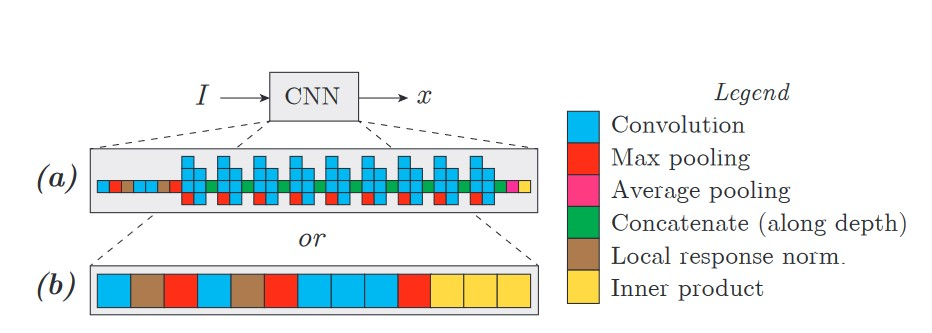
\includegraphics[width=\linewidth]{CNN_image.jpg}
    \caption{CNNs for image embeddings (source \cite{bell2015learning})}
    \label{fig:cnn}
\end{figure}

Further more, another class of popular networks called Siamese offer a better way to handle the embeddings created by CNNs to adapt with the relative similarity and dissimilarity between images by passing them as pairs through the network. This offers a way to build a vector space to find inputs that are similar to each other. Fig. \ref{fig:siamese} shows an outline of simple Siamese network architecture.  

\begin{figure}[H]
  \centering
    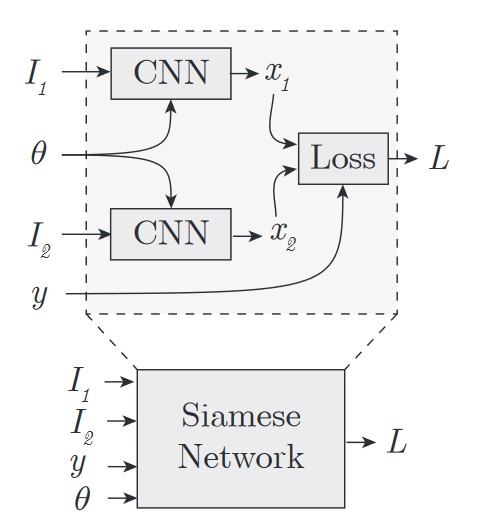
\includegraphics[width=50mm]{siamese_img.jpg}
    \caption{Siamese network architecture (source \cite{bell2015learning})}
    \label{fig:siamese}
\end{figure}

However, the data used to train these Siamese networks may also have classes. Therefore training a Siamese network with both image similarity and also the class labels is also another option. The paper\cite{bell2015learning} achieves this by passing two inputs regarded as similar through a Siamese network and then minimizing the loss from the vector space and also the cross entropy loss of the predicted versus true class labels. After training, the vector space can be visualized using the t-SNE method to see clusters of similar objects at different regions.

In this project we aim to implement the Siamese network proposed in paper \cite{bell2015learning} and apply to our fashion image similarity problem. DeepFashion datasets have abundant data over numerous classes. So for the scope of this project we define our similarity based on the class label of the images. We intend to test different network architectures and losses proposed in the paper and evaluate them on DeepFashion-1 dataset through our main experiments. By evaluation, we calculate the top-K accuracy for queries. We would also use qualitative methods such as visualizing the embedding space and evaluating the quality of retrieved images. At the end, we intend to have an image retrieval or a recommendation engine which can output most similar images to the queried fashion images.

\section{Related work}\label{related_work}
In the last couple of years, a lot of work has been done in the field of image similarity with both different and in most cases similar approaches. Deep convolutional networks have been a central part of this work and has obtained good results. However, this is still an open research field that are still to be fully explored. 

Chaoji et al.\cite{appalaraju2017image} compares a traditional CNN with what they call SimNet to fetch similar looking images using a reference image. SimNet is a Siamese network whose architecture is similar to a Siamese network in \cite{bell2015learning} with a contrastive loss. In their case, the SimNet outperformed the traditional CNN at capturing similarities. 

Wang et al. \cite{wang2014learning} proposed a deep learning model to learn similarity metrics from the images using a specific triplet sampling algorithm to train. The sampling algorithm samples a query image, a positive and a negative match. This approach was shown to outperform models with hand-crafted features. 

A very similar approach to Wang et al.\cite{wang2014learning} was done by Philbin et al. \cite{schroff2015facenet} where they used the same triplet idea to create an embedding from face images to fetch face-similarities. They obtained very good results, in some cases 99 \% accuracy. 

Melekhov et al. \cite{melekhov2016siamese} proposed a method also using a Siamese network to find matching and non-matching pair of images. The method had promising results and it was also shown that a contrastive loss works well with Siamese networks.

It is clear that Siamese networks in general has been proven to work well in this field and problem. For our work, we will focus Siamese networks that are considered to be successful by Bell et al. \cite{bell2015learning}. In this work they explore different types of Siamese networks on image-object similarity by learning an embedding to fetch similar images. These different Siamese architectures are mainly based on architectures given by Razavian \cite{sharif2014cnn} Chopra \cite{chopra2005learning} Wang \cite{wang2014learning} Weston \cite{weston2012deep}. We will investigate on what architectures performs best trained with fashion-data.

\section{Problem description}
In this project we intend to explore the open research field of Image Similarity. We intend to return clothing image results that have high similarity to a fashion image query. In order to achieve this we intend to study how well the embedding space can cluster similar items and separate dissimilar items using different networks and training losses. DeepFashion datasets are recommended for this project.

\section{ Methodology \& Implementation}\label{methods}

We aim to achieve the following for our project:

\begin{itemize}
    \item Train a similarity vector space where similar fashion images are clustered together and different fashion images are separated away
    \item Input unseen fashion images on our similarity vector space trained on Siamese network to obtain similar fashion images.
    \item Explore the trained similarity vector space and see how it changes with various loss function and model architectures of the Siamese network.
    \item Experiment first with simpler dataset to verify the robustness of implementation.
    \item Further train our Siamese network with more class labels and complex dataset to check if it is still able to create a reasonable similarity vector space.
    \item Evaluate different methods by visualizing the vector space obtained and qualitative analysis of top-K similar images.

\end{itemize}  In the following sections, we explain our implementation methods, detailed information of our Siamese network, results and further discussion.

Our Siamese network uses the contrastive loss described in \cite{bell2015learning}. It comprises two loss components, one loss for similar input pair and another loss for dissimilar input pair. These are described in (\ref{eq:1}), (\ref{eq:2}) and (\ref{eq:3}).

\begin{equation}
    L=\sum_{(x_p,x_q)}L_p(x_p,x_q) + \sum_{(x_q,x_r)}L_r(x_q,x_r)\label{eq:1}
\end{equation}
\begin{equation}
    L_p(x_p,x_q)=\left\Vert x_p - x_q \right\Vert^2_2\label{eq:2}
\end{equation}
\begin{equation}
    L_r(x_q,x_r)=max(0, m^2-\left\Vert x_q - x_r \right\Vert^2_2)\label{eq:3}
\end{equation}

\begin{equation}
    L_{ce}=\sum_{i}y_i\log c_i\label{eq:4}
\end{equation}

We give a detailed explanation of the loss function (\ref{eq:1}) as follows. A training sample is made up three image data, $x_q$, $x_p$ and $x_r$, where the first two are images with the same class label and the third is an image with a dissimilar class label. We pass these images into the network and embed them into the embedding space, with the objective of minimising the distance between the similar images and maximising the distance between the dissimilar images with a margin  $m$. As the training progresses, this loss function should guide the formation of an embedding space with similar images clustered together and dissimilar images separated from one another. Even though the class of two images is the same, contrastive loss includes the distance between the image embeddings. This still guides highly similar images even within the same class closer compared to relatively dissimilar intra-class images. This especially is useful when we train considering entire class label as a similarity flag. In one of our networks, we use cross-entropy loss (\ref{eq:4}) for both images in the pair along with the contrastive loss (\ref{eq:1}). In order to make use of both losses, our network outputs both image embeddings ($x_p$, $x_q$, $x_r$) and image class predictions ($c_i$). These losses are summed together to give a final loss that is used to train the networks C and D.

We extended the \textit{Dataset} class of pyTorch to customize it to handle Fashion-MNIST and DeepFashion datasets. We generate fixed pairs positive and negative pairs for testing. And for training we generate random and balanced positive and negative pairs of images. Since we use customized loss, our true labels include individual labels of the image and the combined similarity label of the pair.

\begin{figure}[H]
  \centering
    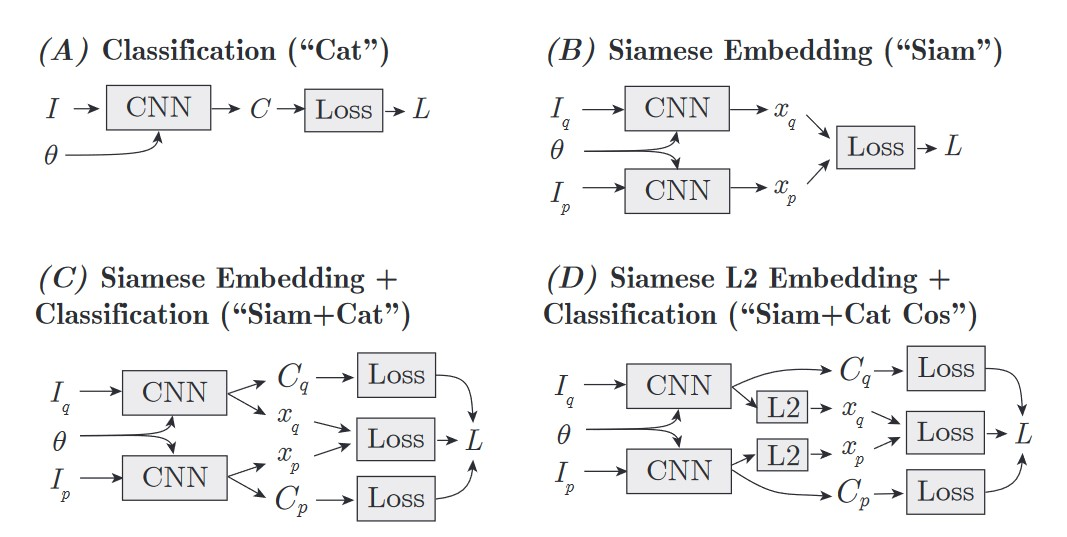
\includegraphics[width=\linewidth]{network_images.jpg}
    \caption{Training Architectures (source \cite{bell2015learning})}
    \label{fig:netwrok_arch}
\end{figure}

%\section{Implementation}
Our network implementations are done using PyTorch and training was on Google Cloud P100/K8 GPUs. A total of four networks were implemented, their architectures are shown in figure \ref{fig:netwrok_arch}. We will call them (A), (B), (C) and (D) as in figure \ref{fig:netwrok_arch}. The datasets used and the experiments will also be explained in this section.

\subsection{Network Architectures}
Here, all networks will be described. The complexity of the architectures increases from (A) to (D), as seen in figure \ref{fig:netwrok_arch}. The first network (A) is the most primitive network that we implemented and works like a traditional CNN for classification. We tried pre-trained ResNet-18/34/50 that we fine-tuned with DeepFashion-1 dataset. We used the penultimate layer to extract the embeddings for the similarity space. The network (B) works like a traditional Siamese network, with shared model parameters and one loss function. The model was trained with samples of a positive pair and a negative pair where a pair is considered positive if the two images are from the same class. We used the contrastive loss function for this network. We experimented with ResNet-18/34 as base CNNs for this model. The network C is almost like B, the only extension are that it has three loss functions instead of one. Here we try to predict the class of the both images and both cross-entropy losses are added to the contrastive loss. Network (D) is a extended version of C where L2 regularisation is added to embeddings.

\subsection{Dataset}
Models were initially tested with simpler Fashion-MNIST \cite{xiao2017/online} dataset. It contains gray-scale fashion images of $28\times28$ dimension and has 10 classes. After we concluded that this dataset worked for our networks, we proceed to use DeepFashion-1 \cite{liuLQWTcvpr16DeepFashion} for our main experiments. DeepFashion-1 contains around 289K images consisting of 46 different classes. With classes being highly imbalanced, we re-sampled the data to obtain 5000 images each for top 15 classes. Moreover, images have only one dimension fixed to 300. So every image has been resized accordingly to fit the networks used. 

\begin{figure}[H]
  \centering
    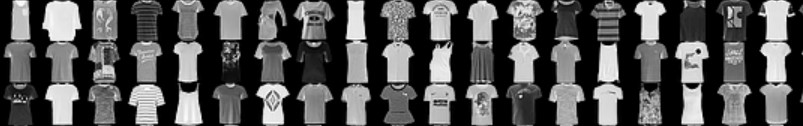
\includegraphics[width=\linewidth]{fmnist.jpg}
    \caption{Samples from Fashion-MNIST Dataset}
    \label{fig:fmnist}
\end{figure}

\begin{figure}[H]
  \centering
    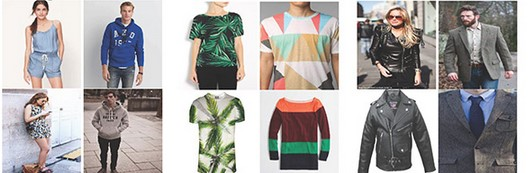
\includegraphics[width=\linewidth]{dfimages.jpg}
    \caption{Samples from DeepFashion-1 Dataset}
    \label{fig:df}
\end{figure}

\section{Experiments \& Evaluation}

Our initial experiments were on Fashion-MNIST dataset so that we could verify the entire pipeline of training a simple neural network is working. Then we used it to create a similarity space, obtain embeddings of all images and visualize them. Finally, we performed similar image retrieval on that. We used a simple CNN with two convolutional layers and two fully connected layers resulting in 256D embeddings as our base model in Siamese for Fashion-MNIST.

Next we worked with DeepFashion dataset by experimenting on all four networks. We realized to be able to compare models we need each of them individually well tuned to hyper-parameters. For a robust implementation we tried different hyper parameters which included different margin size in the contrastive loss along with other usual hyper parameters. Very large margins in contrastive loss can lead to diverging results and too small can lead to slow learning. Considering the heavy ResNet serving as base network for our Siamese models, each training session takes considerable amount of time and compute. We used pretrained weights initialization for our base ResNets. These weights are from training on ImageNet dataset. 

\subsection{Visualization}
After training we should obtain an embedding space representing images, and as we trained using class labels as the similarity indicator it is expected that we obtain clusters of the classes in the embedding. This is hard to visualise with 512 and 2048 dimensions. T-distributed stochastic neighbor embedding (t-SNE) is a algorithm in machine learning that is well suited to represent high-dimensional data in low-dimensional space which we used. By packing similar objects with a higher probability the algorithm can lower the dimension in the representation. In the embedding we obtain, t-SNE is used to visualize the embedding space for us to evaluate if fine clustered data are formed.

\subsection{Nearest Neighbours}
Once we have a trained model, we aim to fetch similar images to any of the query images. The first step for this is to obtain embeddings for all the images in the dataset. From our trained models we usually get 512-D vector embedding for each image in case of base network being ResNet-18/34. For ResNet-50 it is 2048-D vector embedding. A naive KNN implementation results in very slow inference. Therefore, we use a python library called \textit{Annoy} \cite{AnnoyGitHub} built for the exact purpose of searching for similar points to a query point in very high dimensional spaces. It performs an approximate nearest neighbour search by first creating an index using a forest of binary trees created by random projections. This is one of the fastest libraries for nearest neighbour search. 

Performing a nearest neighbour search offer us for both qualitative and quantitative evaluation. For quantitative evaluation of the models, we calculate the top-K accuracy based on the class label of top-K nearest neighbours to any query image. And for qualitative evaluation, closest neighbours of the query images can be verified by us manually for similarity.


\subsection{Results}
Here we first showcase our visualization of embedding space obtained from the above described networks. For networks B, C and D we experimented with different margin sizes in the Contrastive loss and we show the best results. Next, we show the top 5 images retrieved for each query image (left most image) in the order from Network A-D. And finally we have images representing the top-50 accuracies per class for each network. We discuss these results in the next section.

\begin{figure}[H]
  \centering
    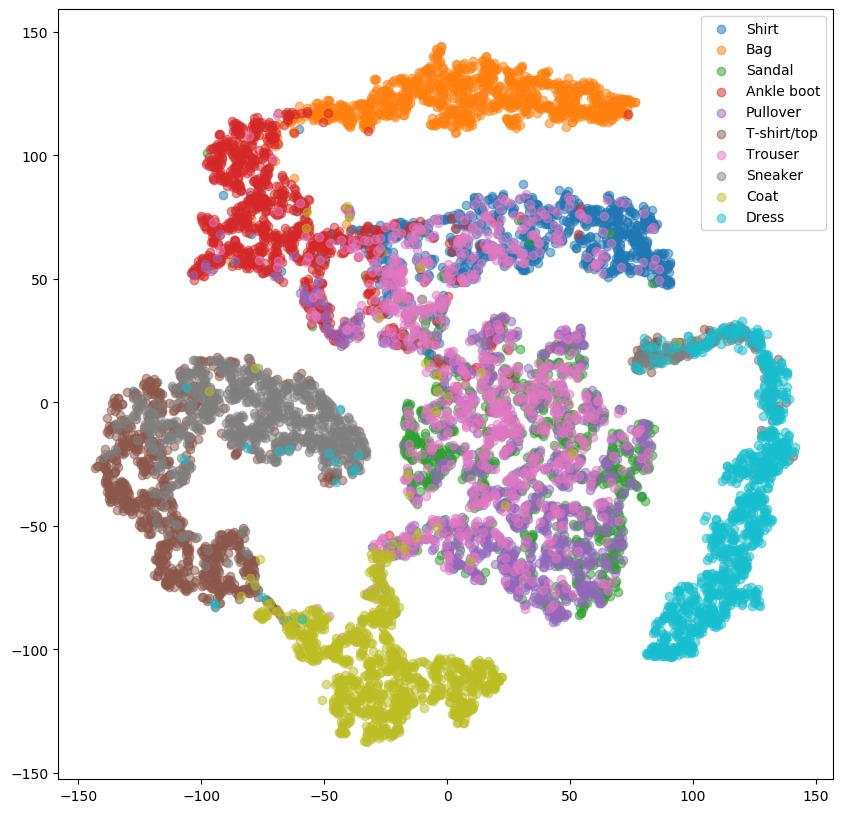
\includegraphics[width=10cm,height=10cm,keepaspectratio]{fashionMnist_viz.jpeg}
    \caption{Clusters from Fashion-MNIST embedding space}
    \label{fig:fmnist}
\end{figure}

\begin{figure}[H]
  \centering
    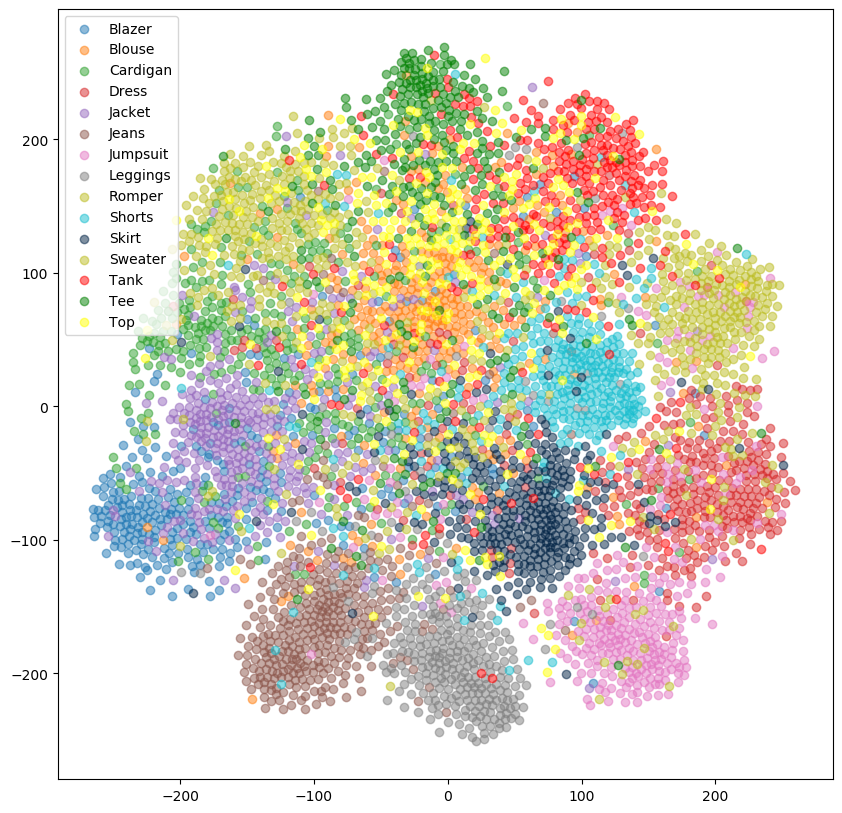
\includegraphics[width=10cm,height=10cm,keepaspectratio]{tSne_Plots/a_t-sne.png}
    \caption{t-SNE Visualization for Network (A)}
    \label{fig:fmnist}
\end{figure}

\begin{figure}[H]
  \centering
    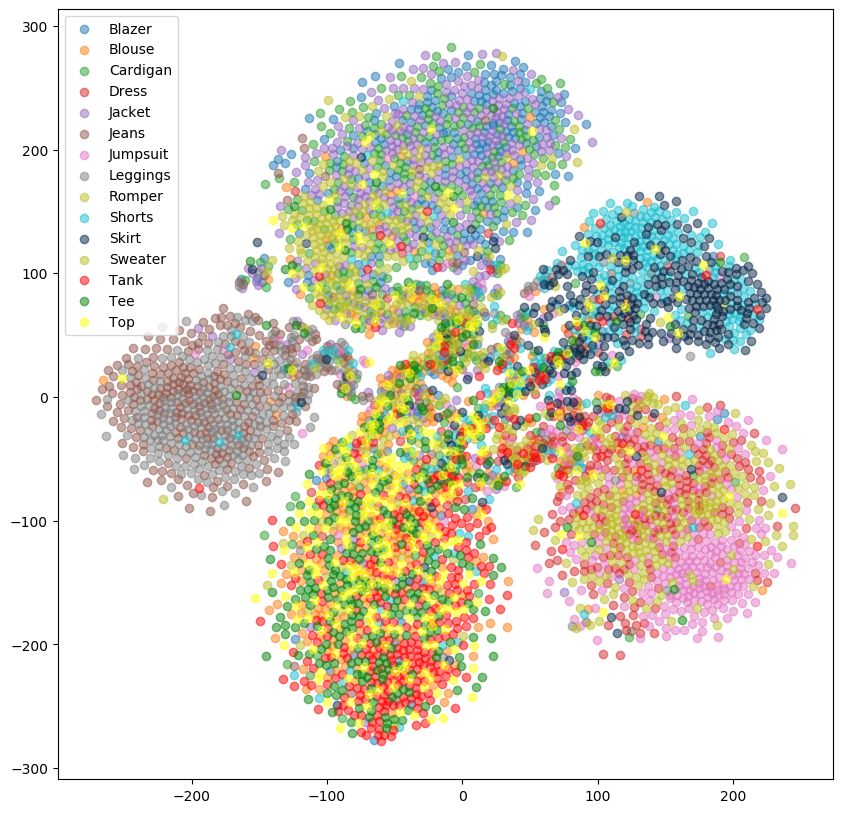
\includegraphics[width=10cm,height=10cm,keepaspectratio]{tSne_Plots/c_100_t-sne.png}
    \caption{t-SNE Visualization for Network (B) with margin=$\sqrt{100}$}
    \label{fig:fmnist}
\end{figure}

\begin{figure}[H]
  \centering
    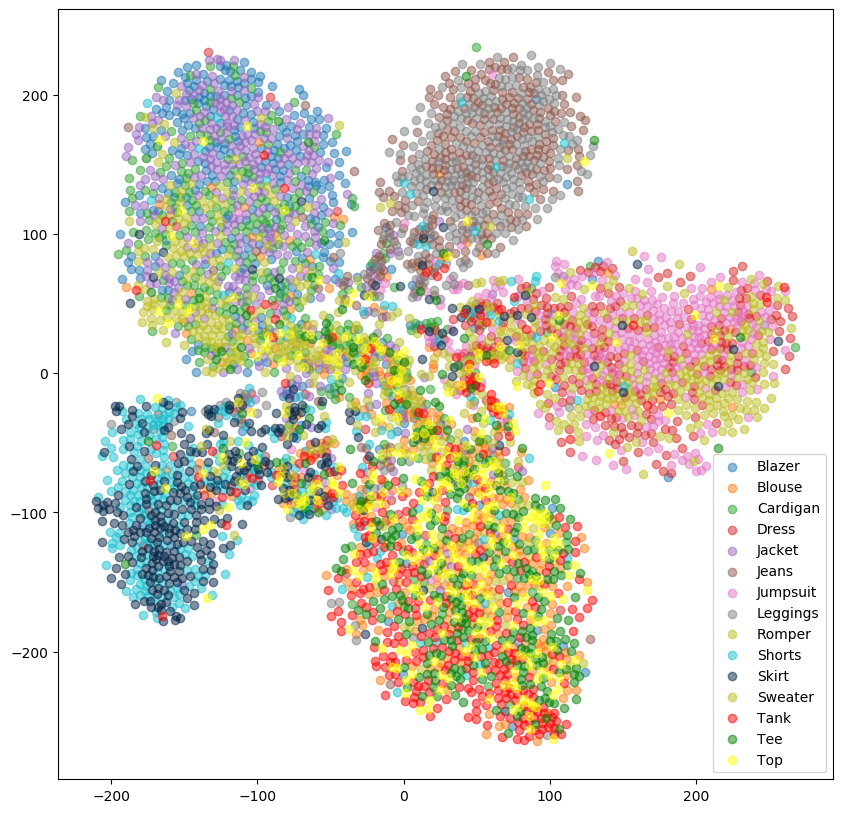
\includegraphics[width=10cm,height=10cm,keepaspectratio]{tSne_Plots/c_1000_t-sne.png}
    \caption{t-SNE Visualization for Network (B) with margin=$\sqrt{1000}$}
    \label{fig:df}
\end{figure}

\begin{figure}[H]
  \centering
    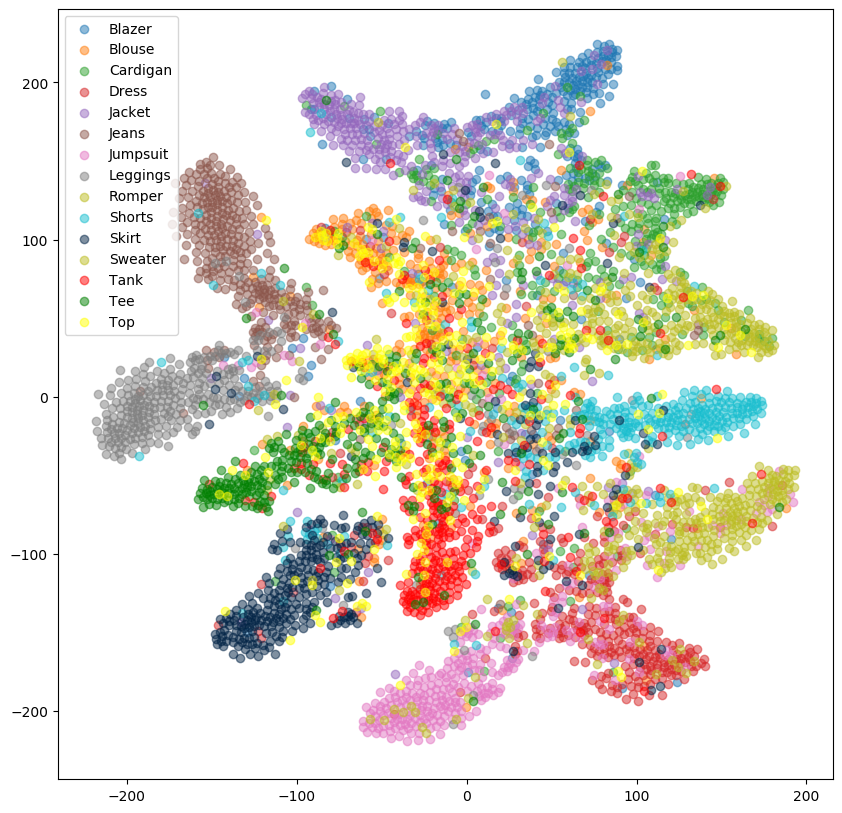
\includegraphics[width=10cm,height=10cm,keepaspectratio]{tSne_Plots/d_100_t-sne.png}
    \caption{t-SNE Visualization for Network (C) with margin=$\sqrt{100}$}
    \label{fig:fmnist}
\end{figure}

\begin{figure}[H]
  \centering
    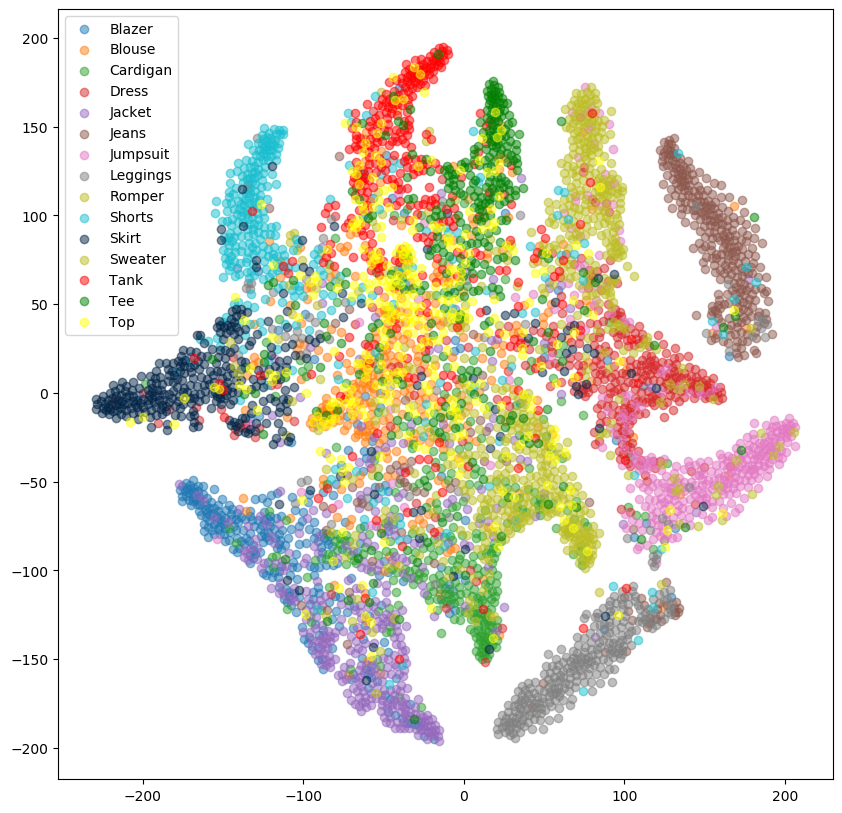
\includegraphics[width=10cm,height=10cm,keepaspectratio]{tSne_Plots/d_1000_t-sne.png}
    \caption{t-SNE Visualization for Network (C) with margin=$\sqrt{1000}$}
    \label{fig:df}
\end{figure}

\begin{figure}[H]
  \centering
    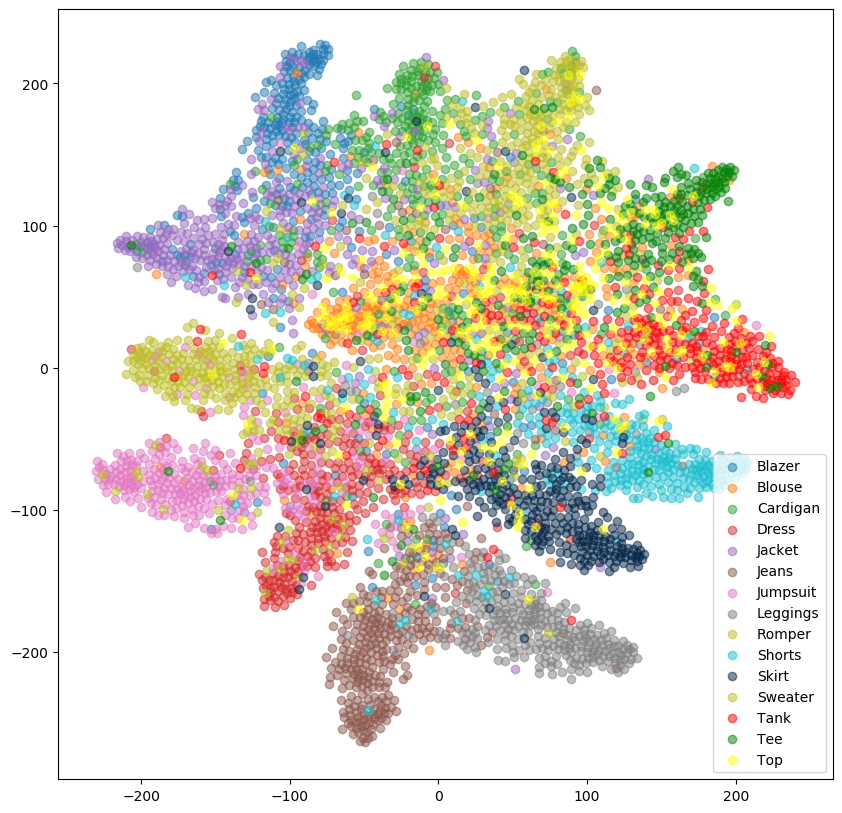
\includegraphics[width=10cm,height=10cm,keepaspectratio]{tSne_Plots/b_t-sne.png}
    \caption{t-SNE Visualization for Network (D) with margin=$\sqrt{0.2}$\\ \\ \\~}
    \label{fig:df}
\end{figure}

\begin{figure}
\begin{tabular}{c}
{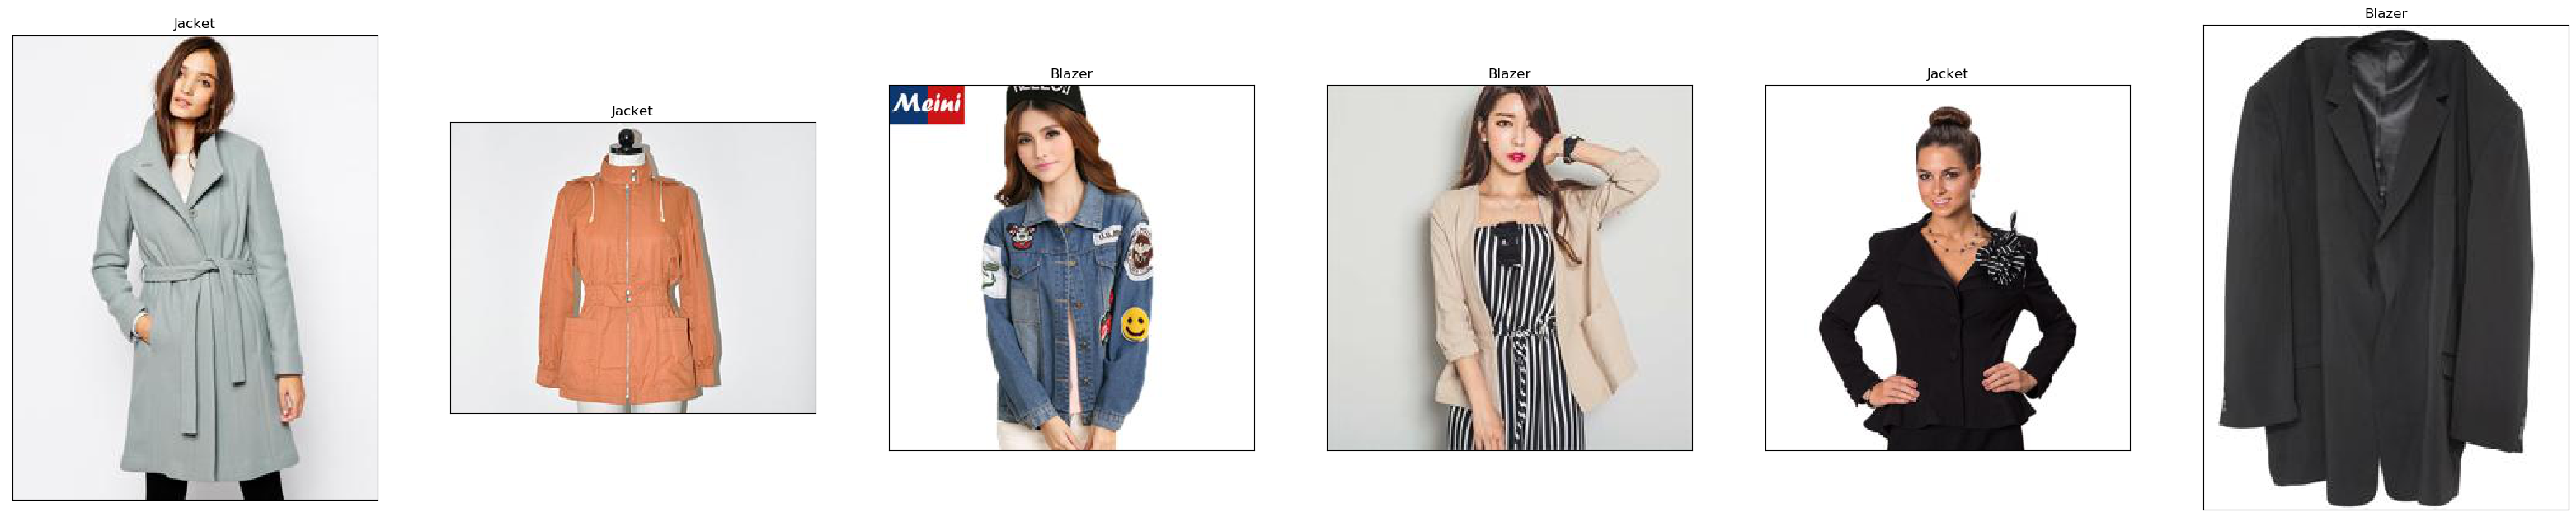
\includegraphics[width = 5in]{a/search_idx_3012.png}}\\
{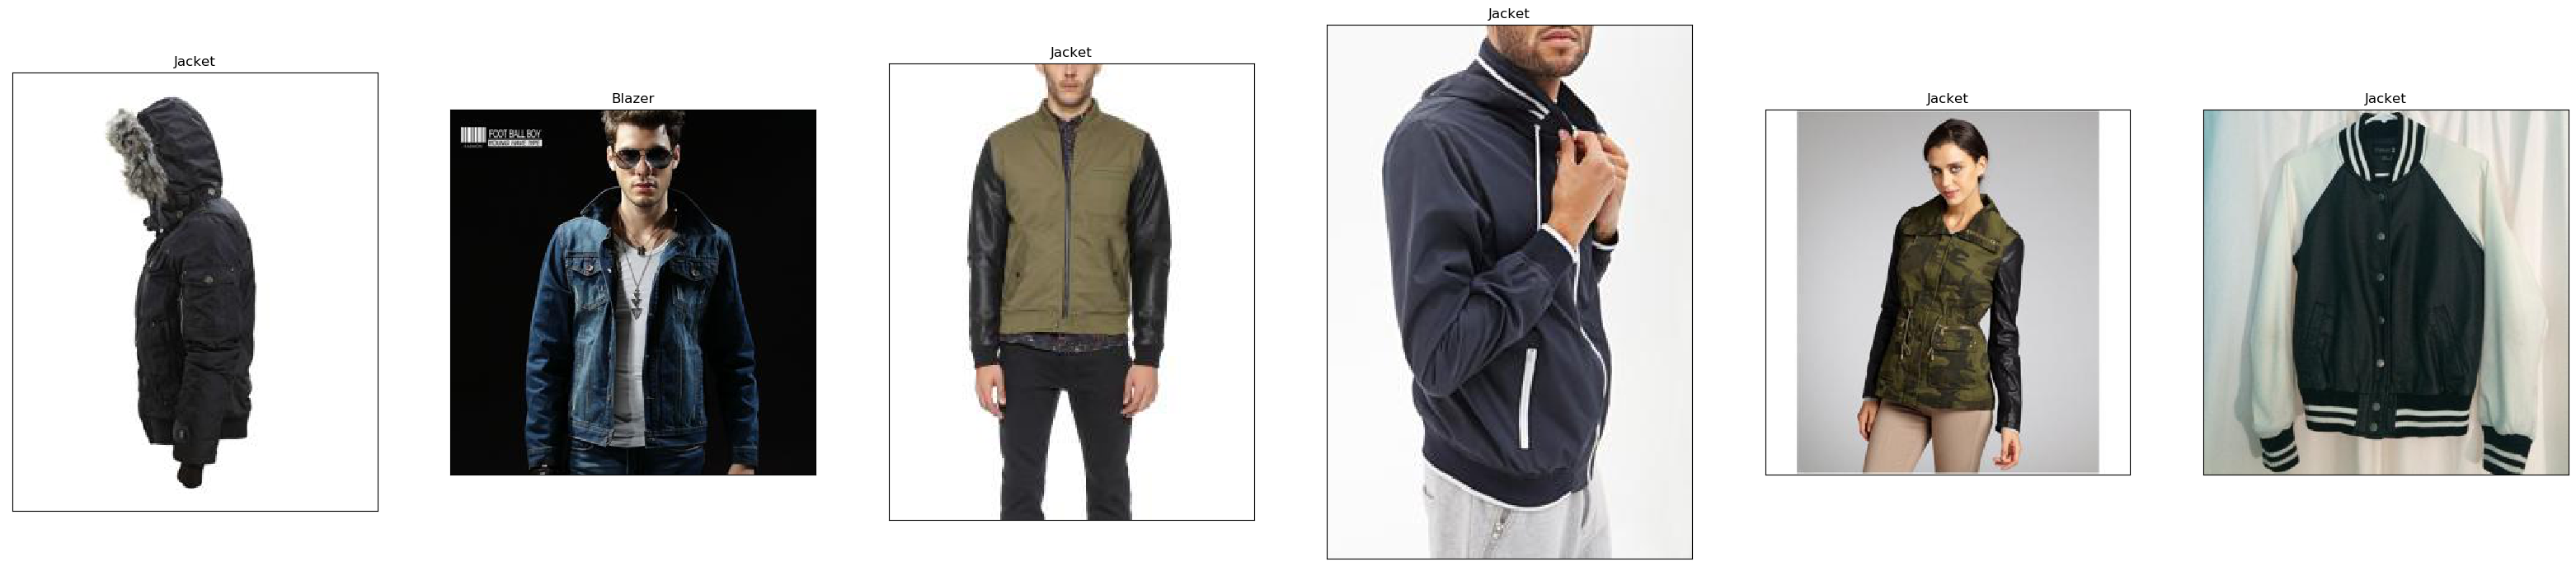
\includegraphics[width = 5in]{a/search_idx_3013.png}}\\
{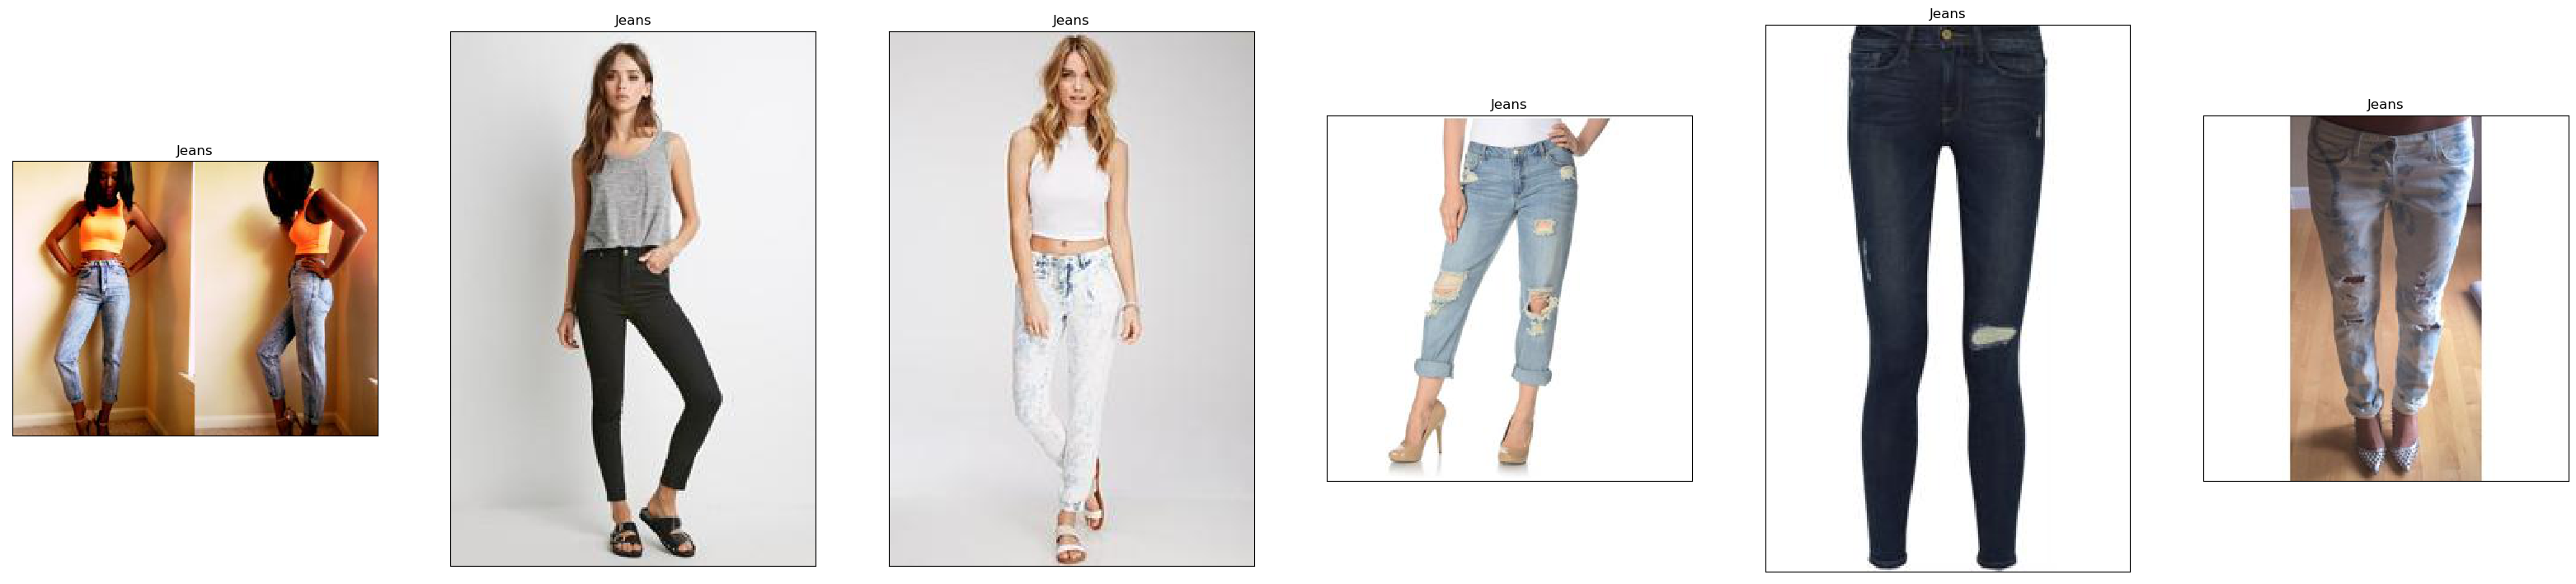
\includegraphics[width = 5in]{a/search_idx_4002.png}}\\
{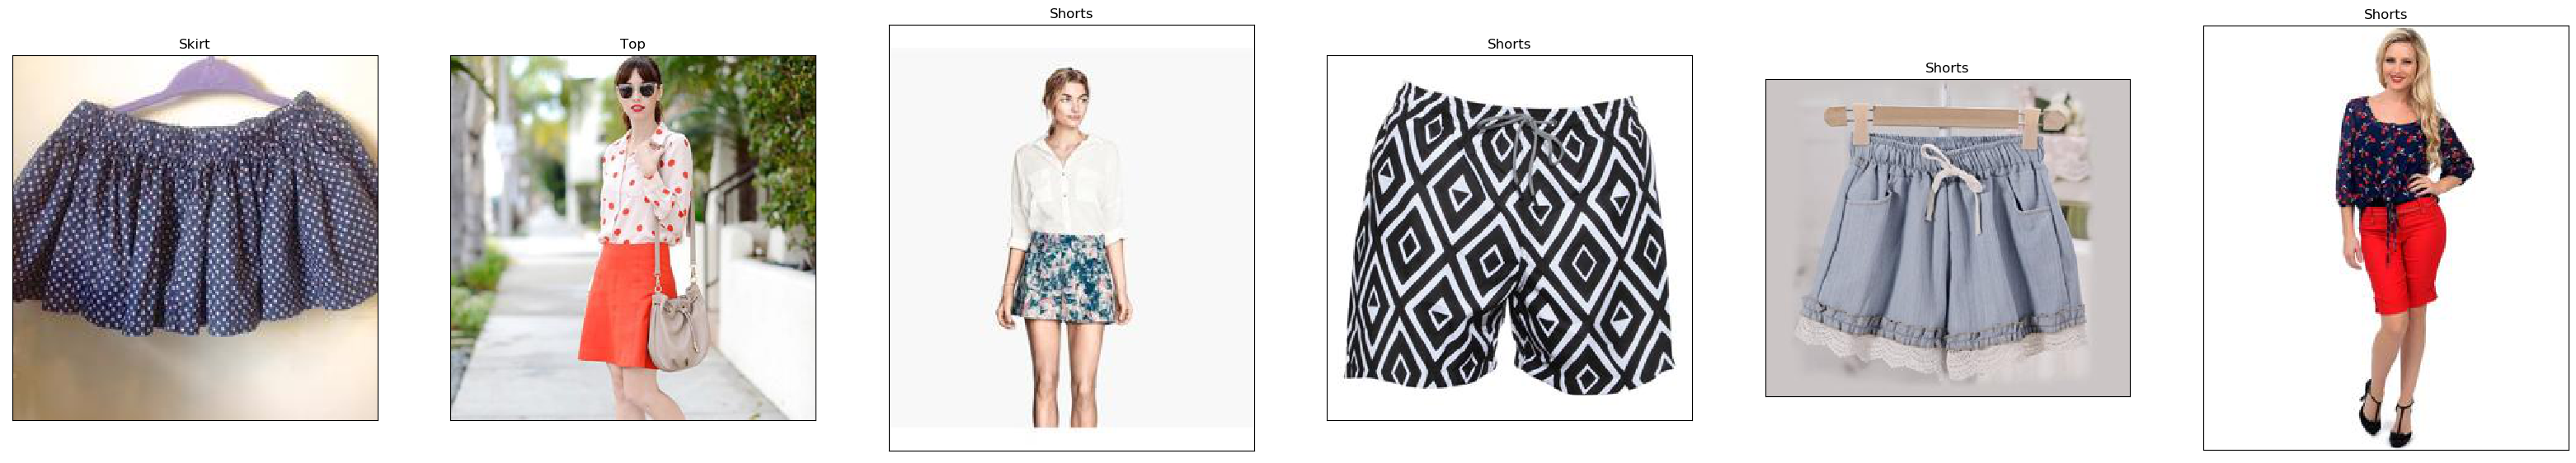
\includegraphics[width = 5in]{a/search_idx_7513.png}}\\
{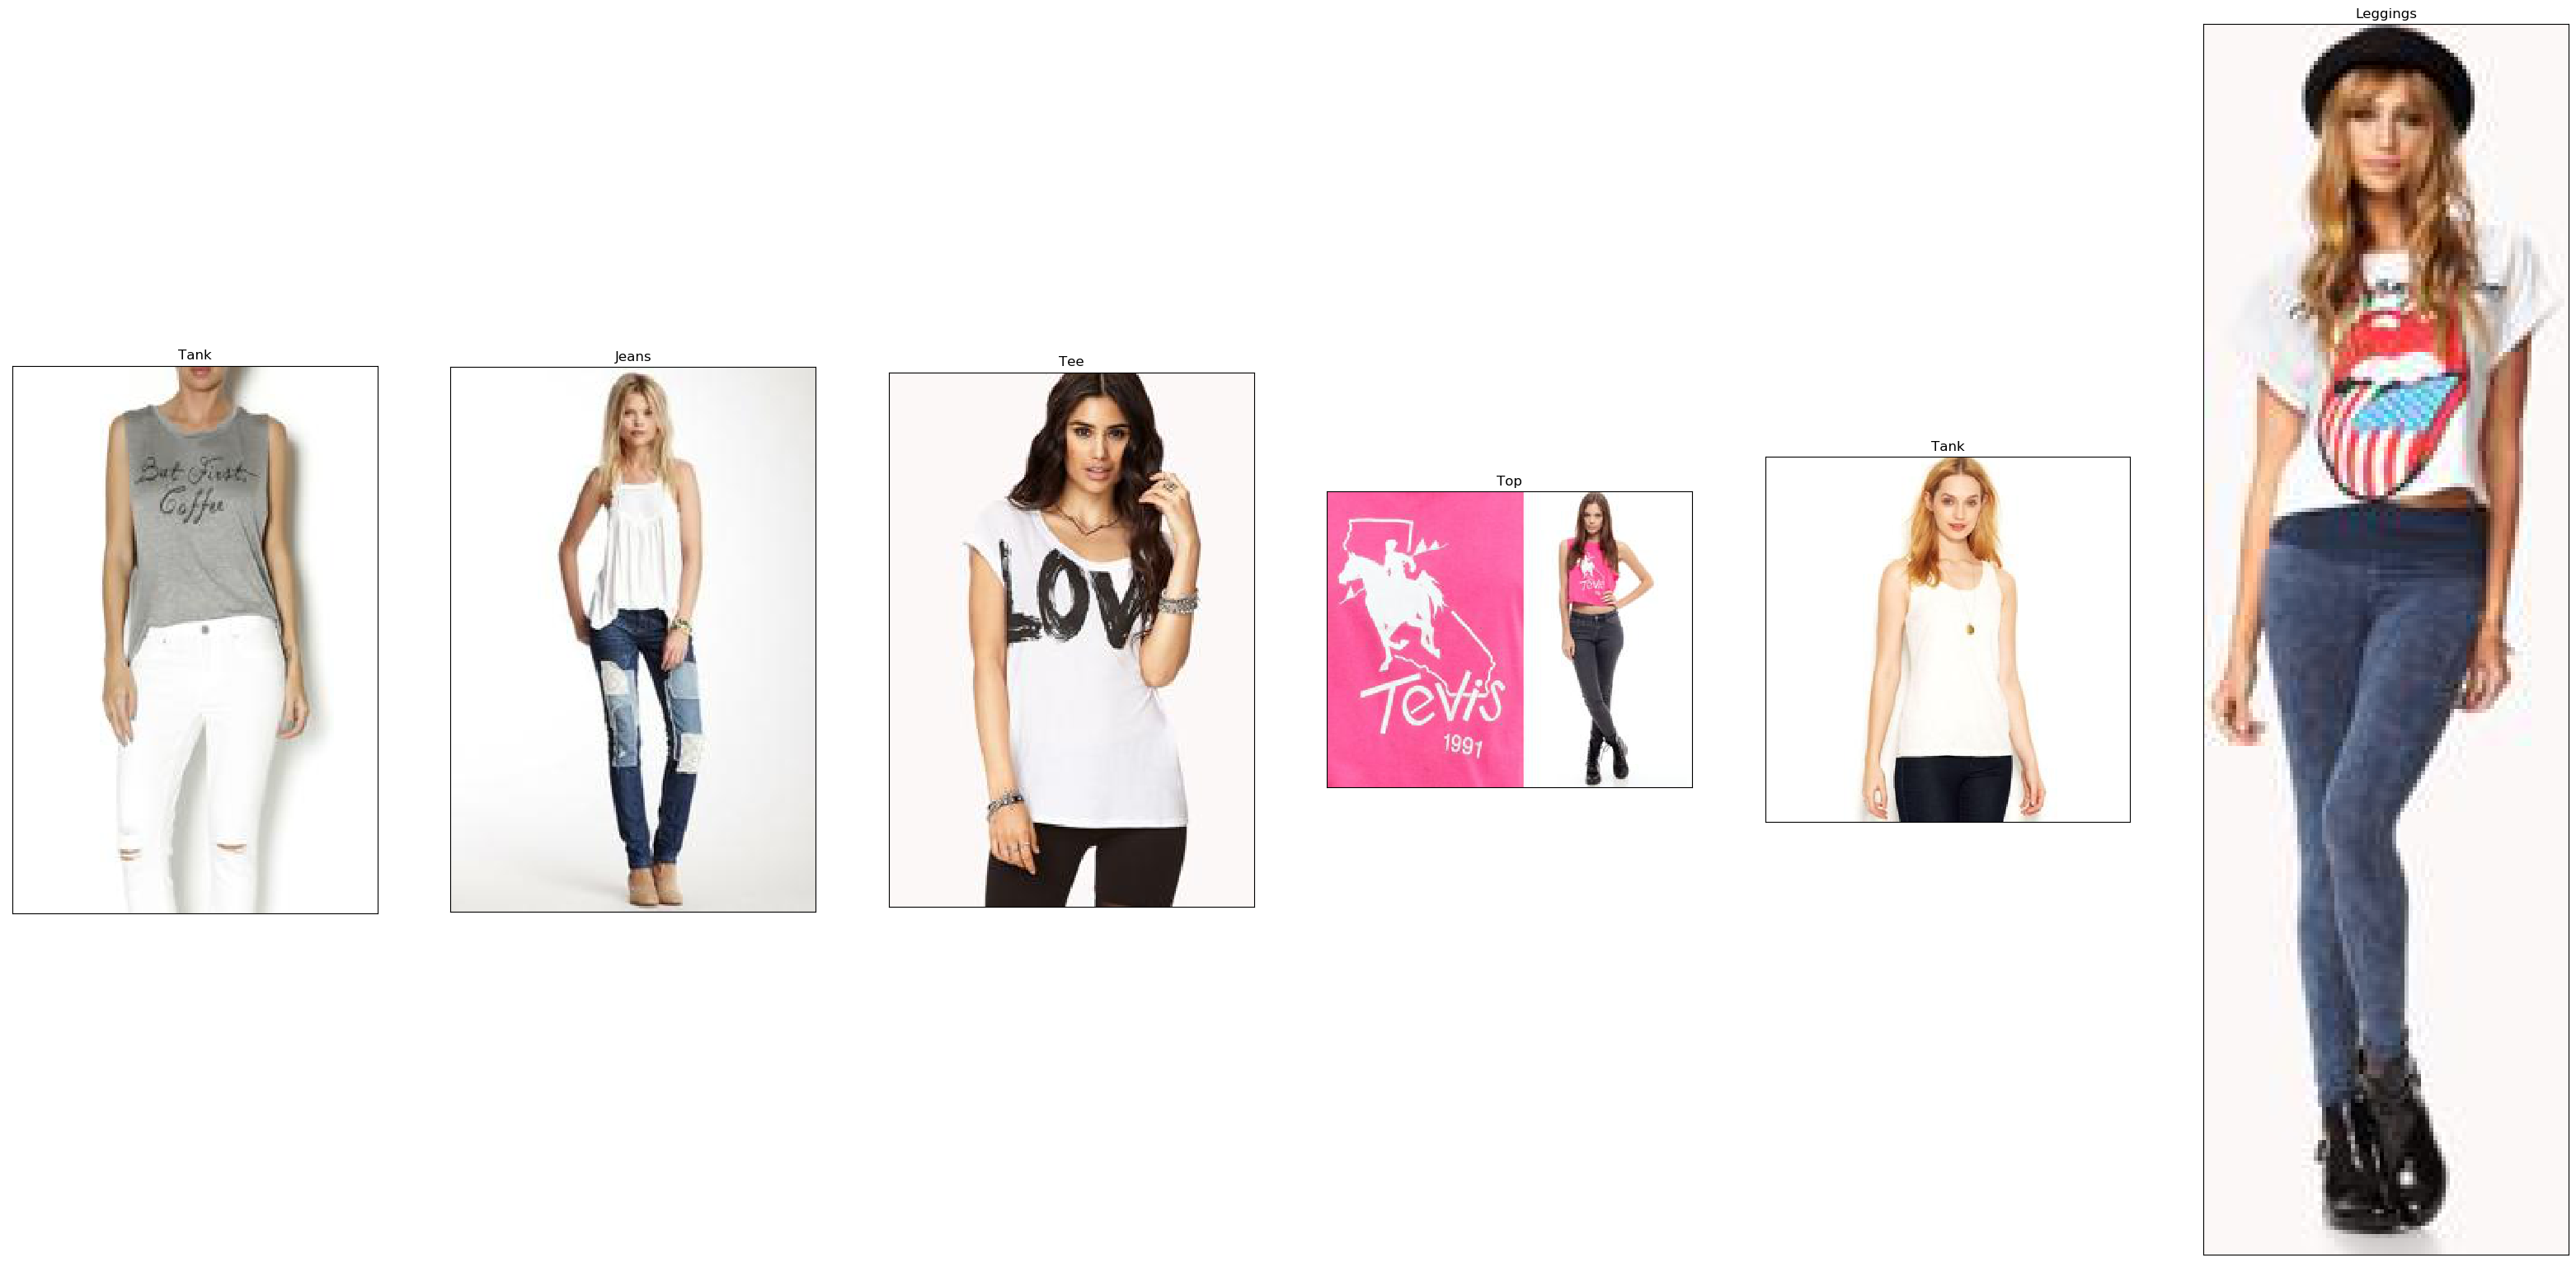
\includegraphics[width = 5in]{a/search_idx_8716.png}}\\
{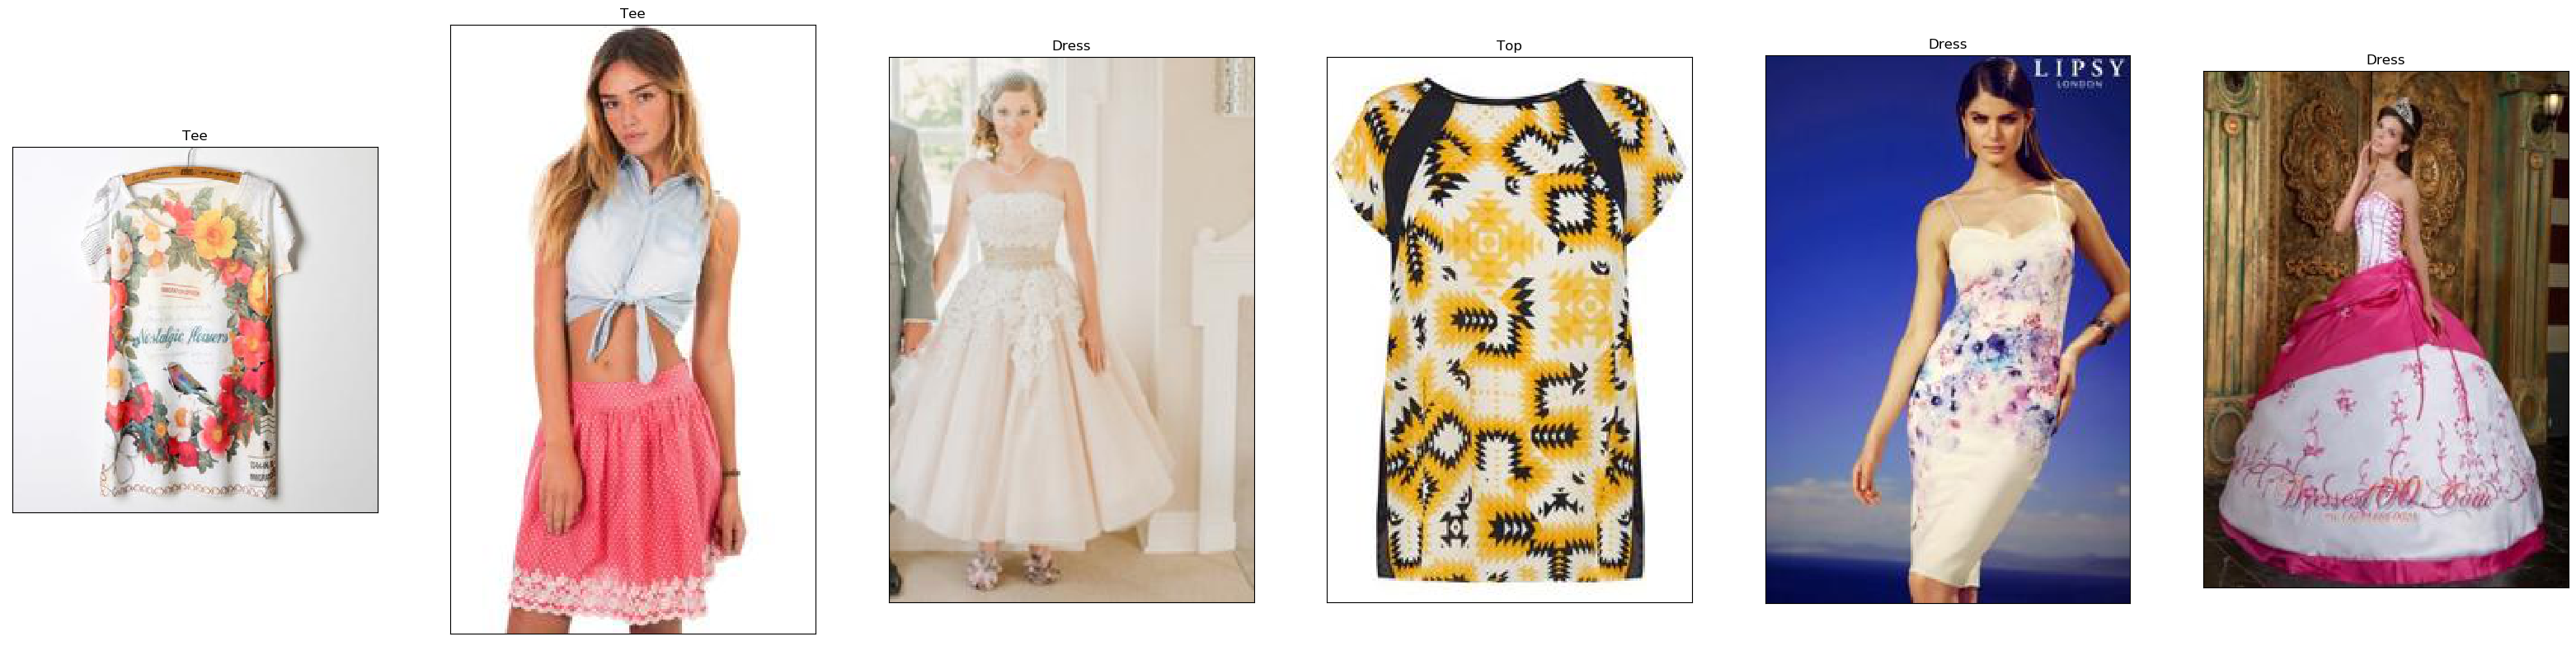
\includegraphics[width = 5in]{a/search_idx_9388.png}}
\end{tabular}
\caption{Top 5 images for Network (A)}
\label{fig:img_netA}
\end{figure}

\begin{figure}
\begin{tabular}{c}
{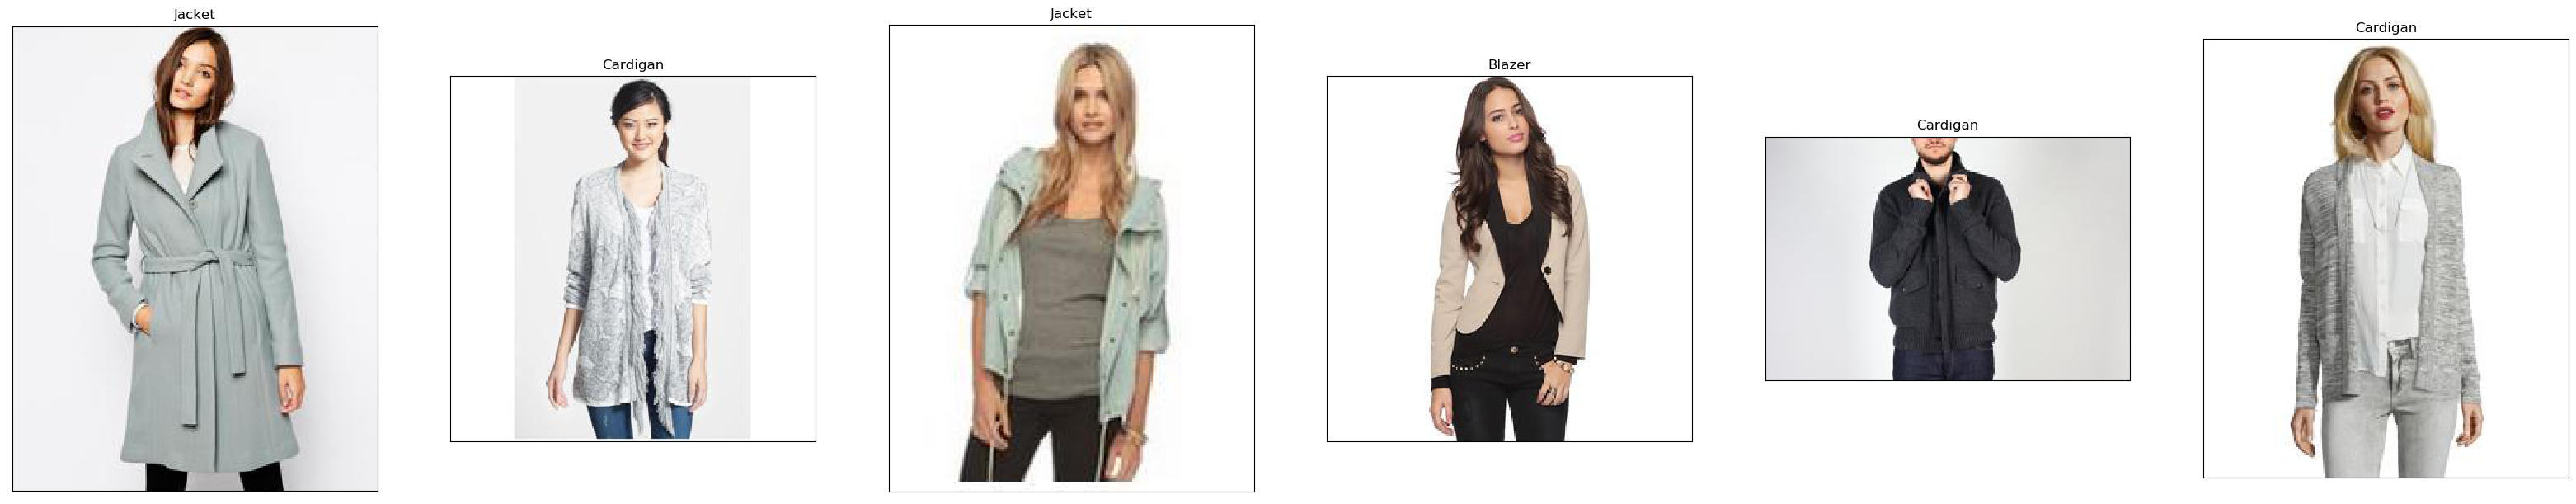
\includegraphics[width = 5in]{b/search_idx_3012.png}}\\
{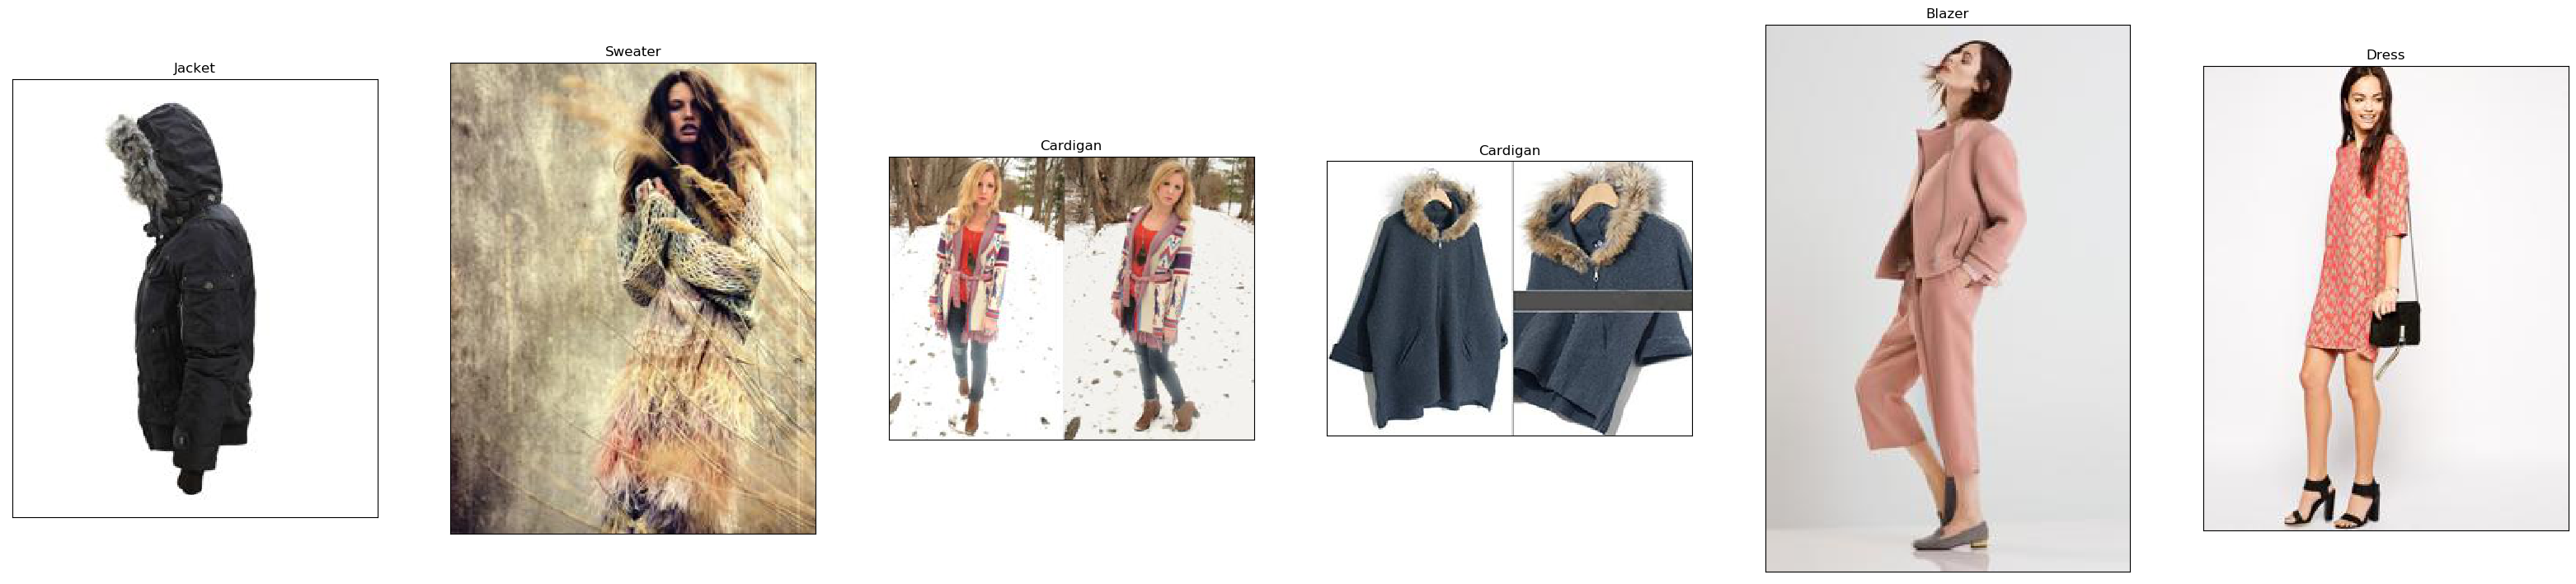
\includegraphics[width = 5in]{b/search_idx_3013.png}}\\
{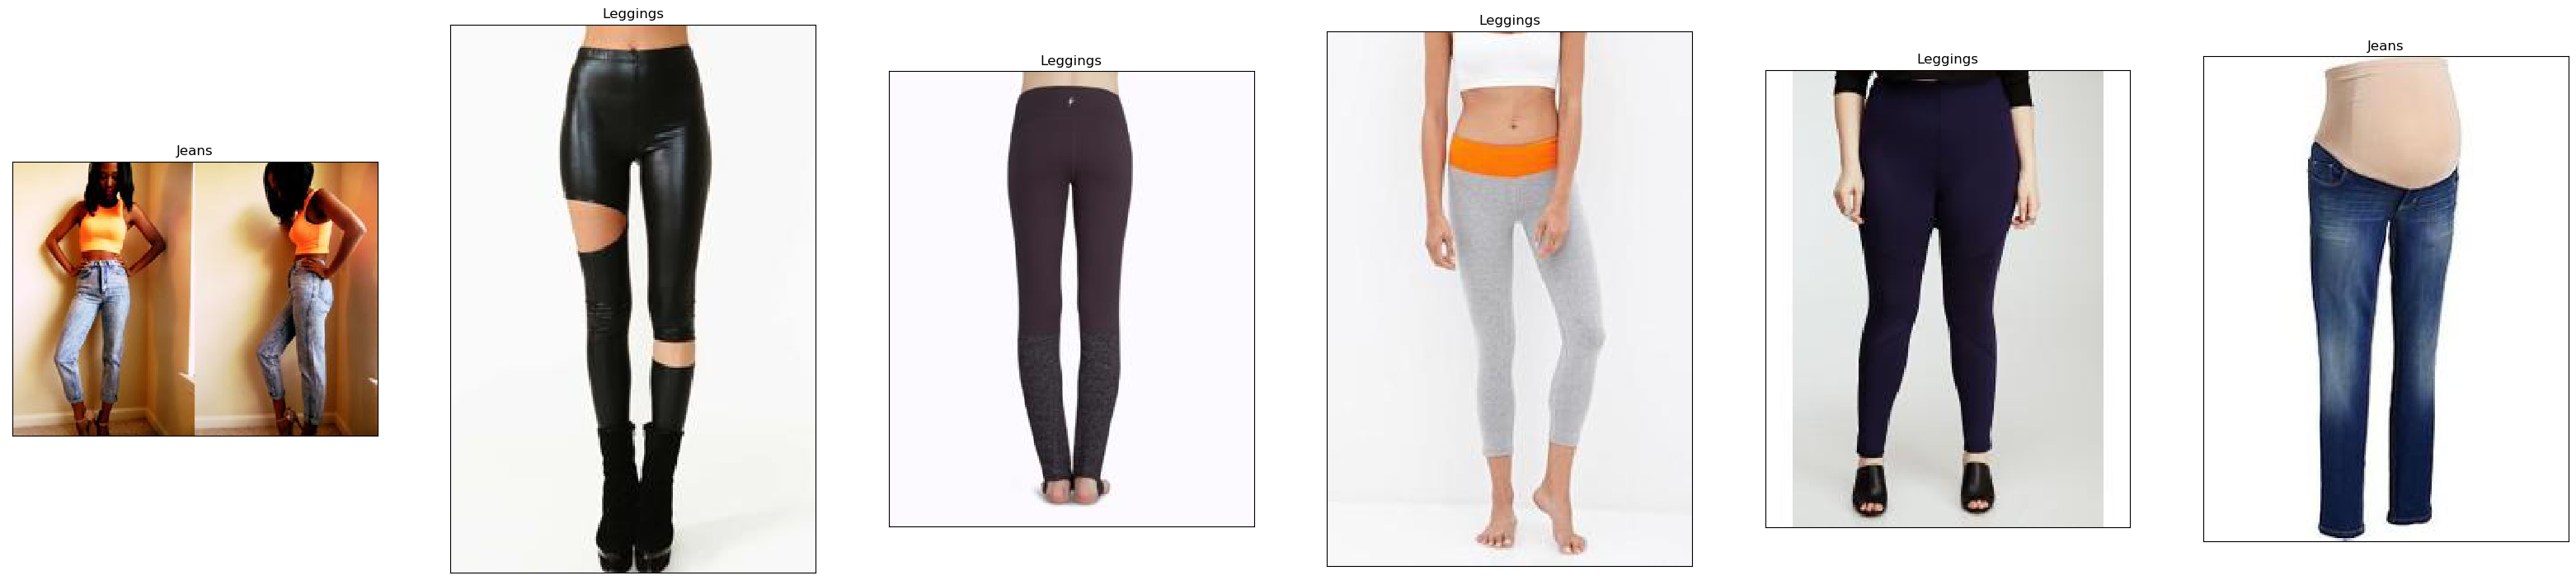
\includegraphics[width = 5in]{b/search_idx_4002.png}}\\
{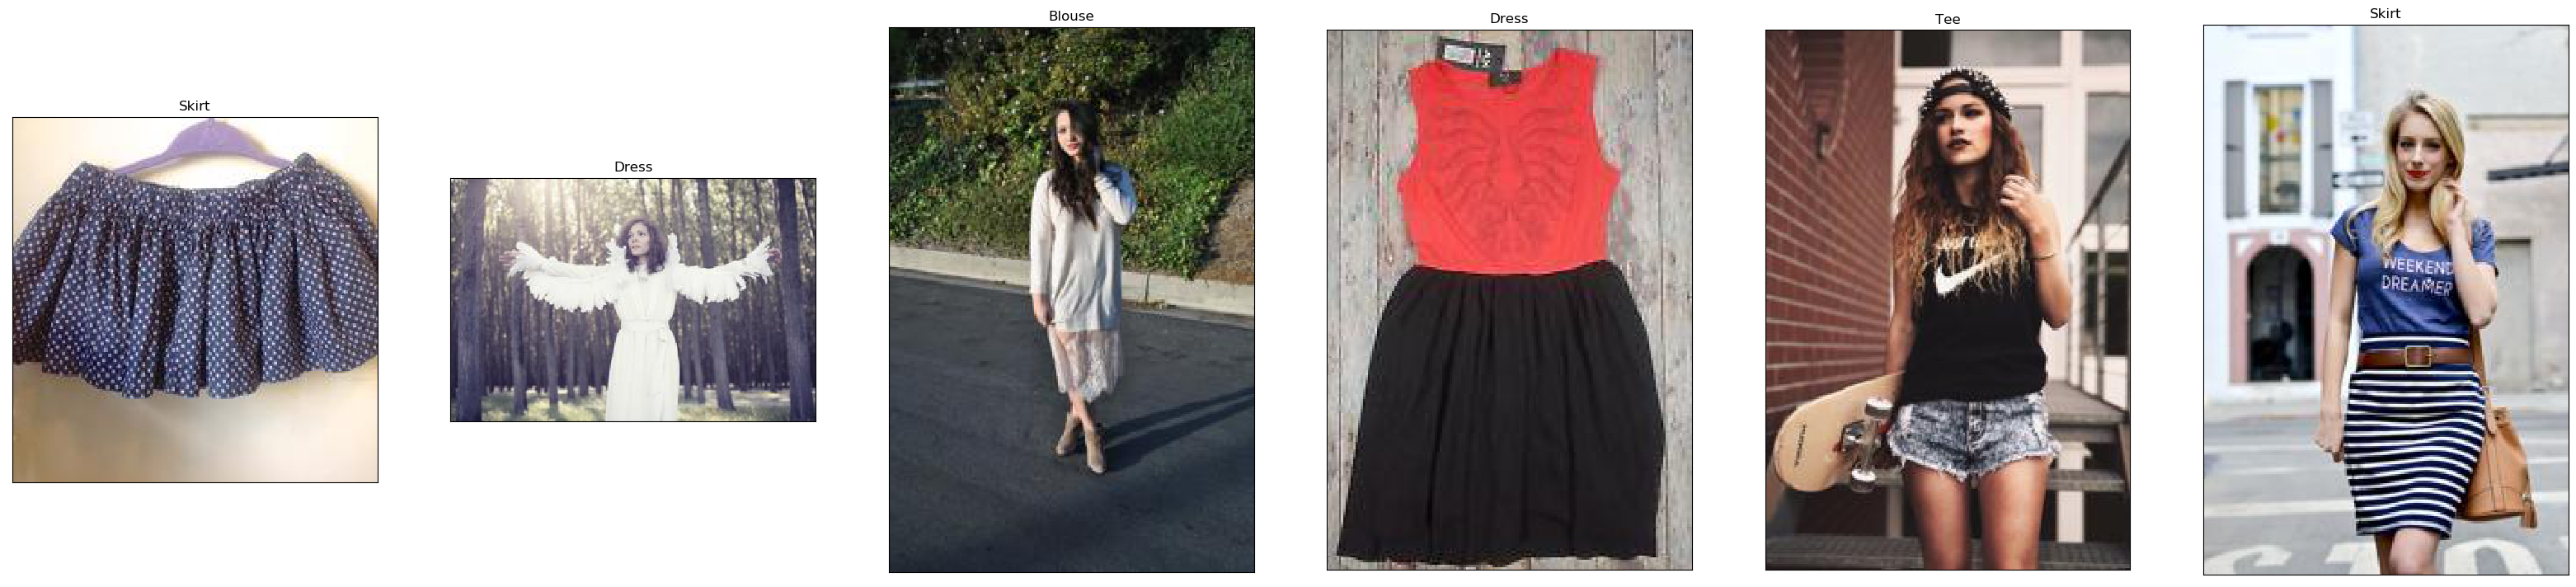
\includegraphics[width = 5in]{b/search_idx_7513.png}}\\
{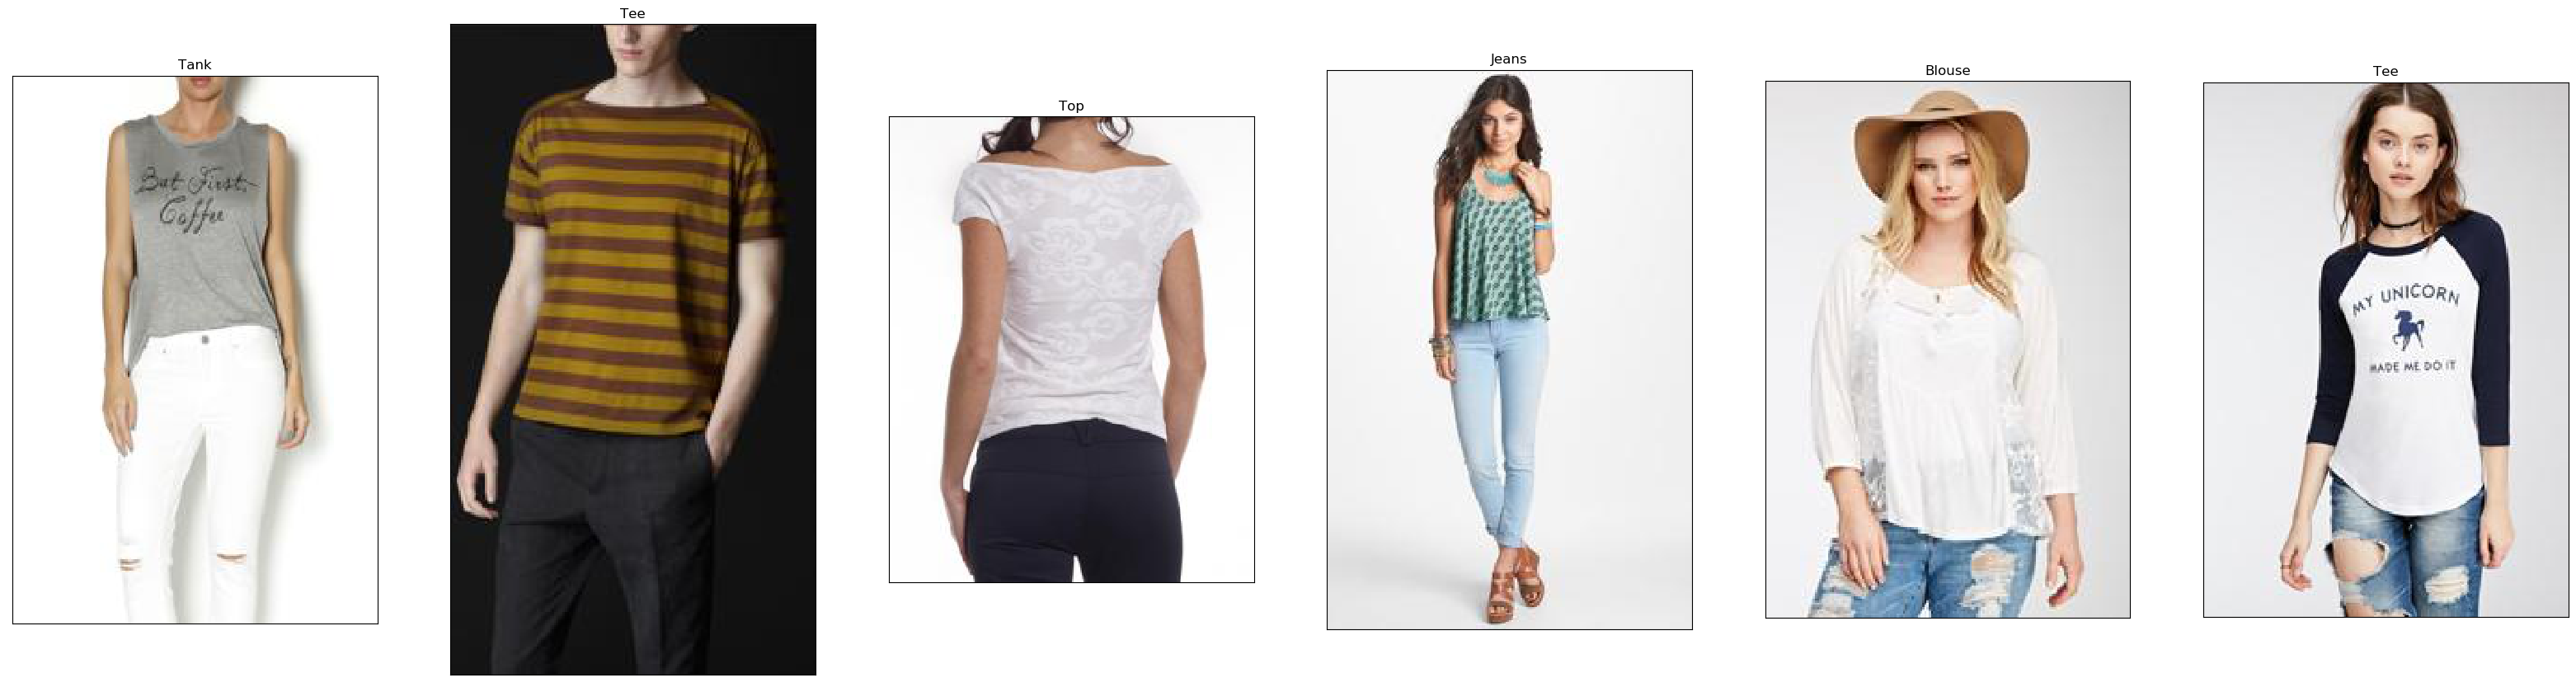
\includegraphics[width = 5in]{b/search_idx_8716.png}}\\
{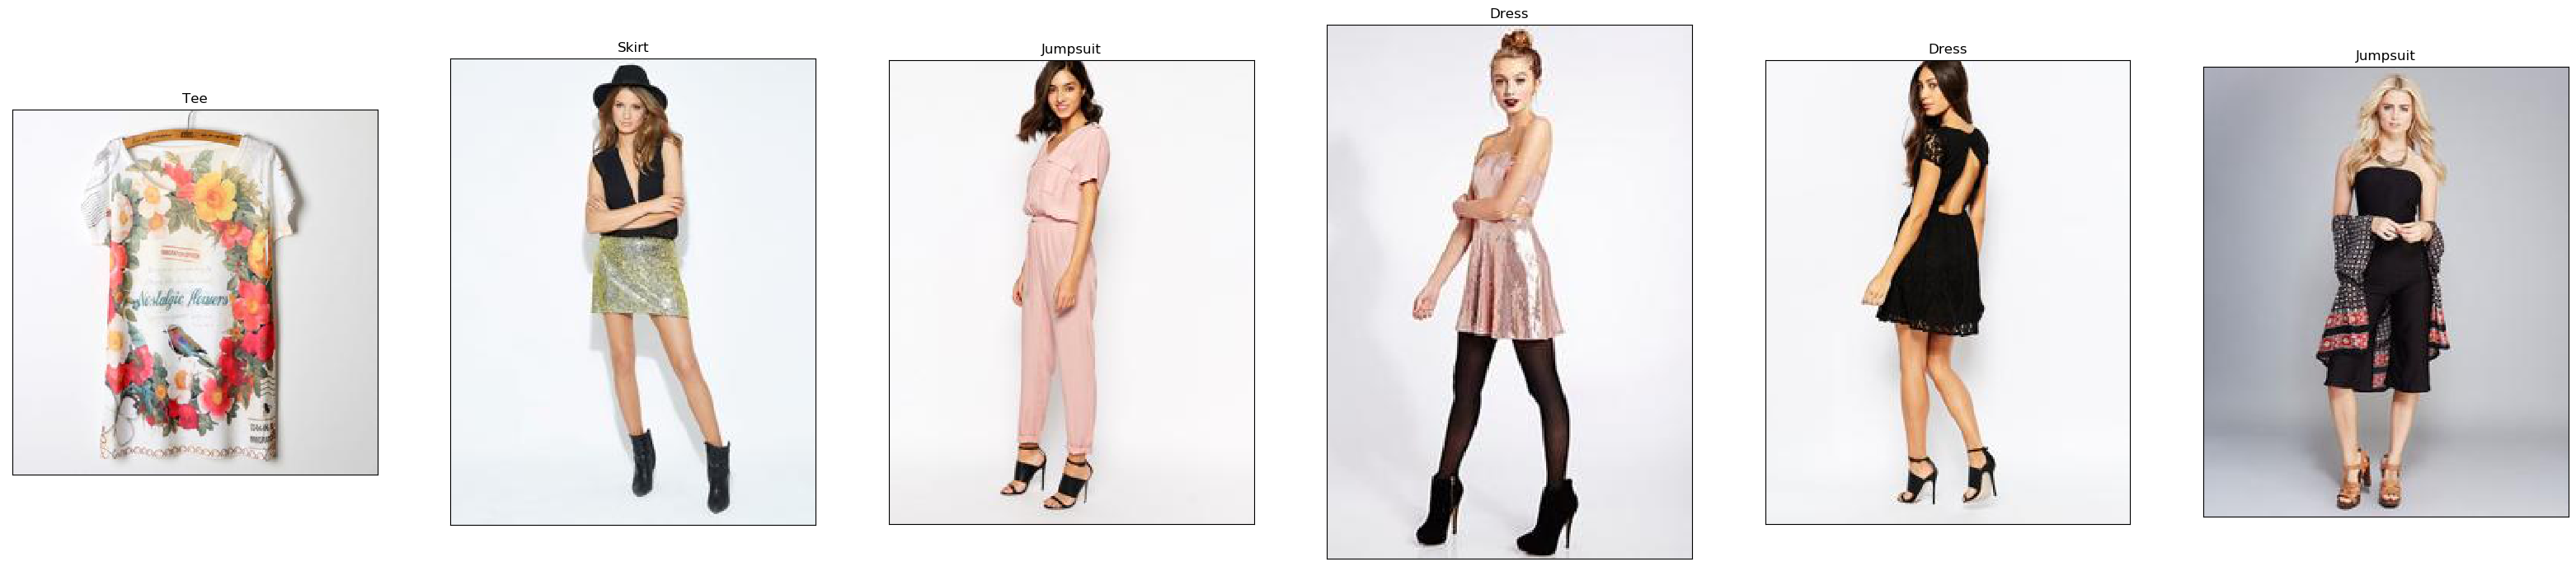
\includegraphics[width = 5in]{b/search_idx_9388.png}}
\end{tabular}
\caption{Top 5 images for Network (B)}
\label{fig:img_netB}
\end{figure}

\begin{figure}
\begin{tabular}{c}
{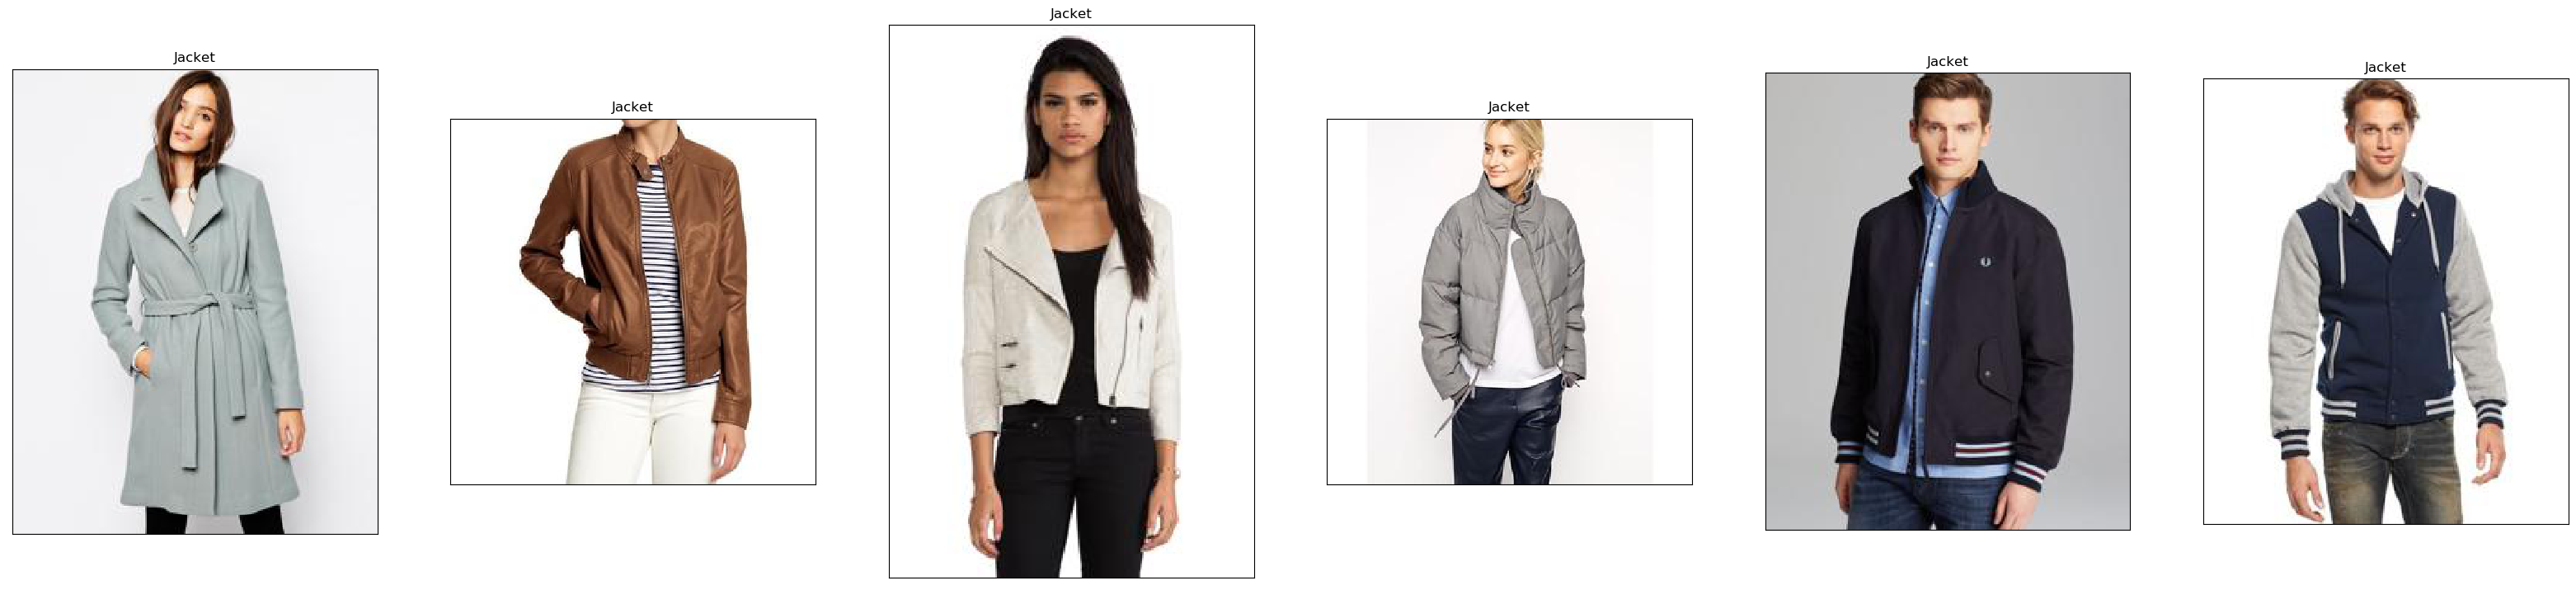
\includegraphics[width = 5in]{c/search_idx_3012.png}}\\
{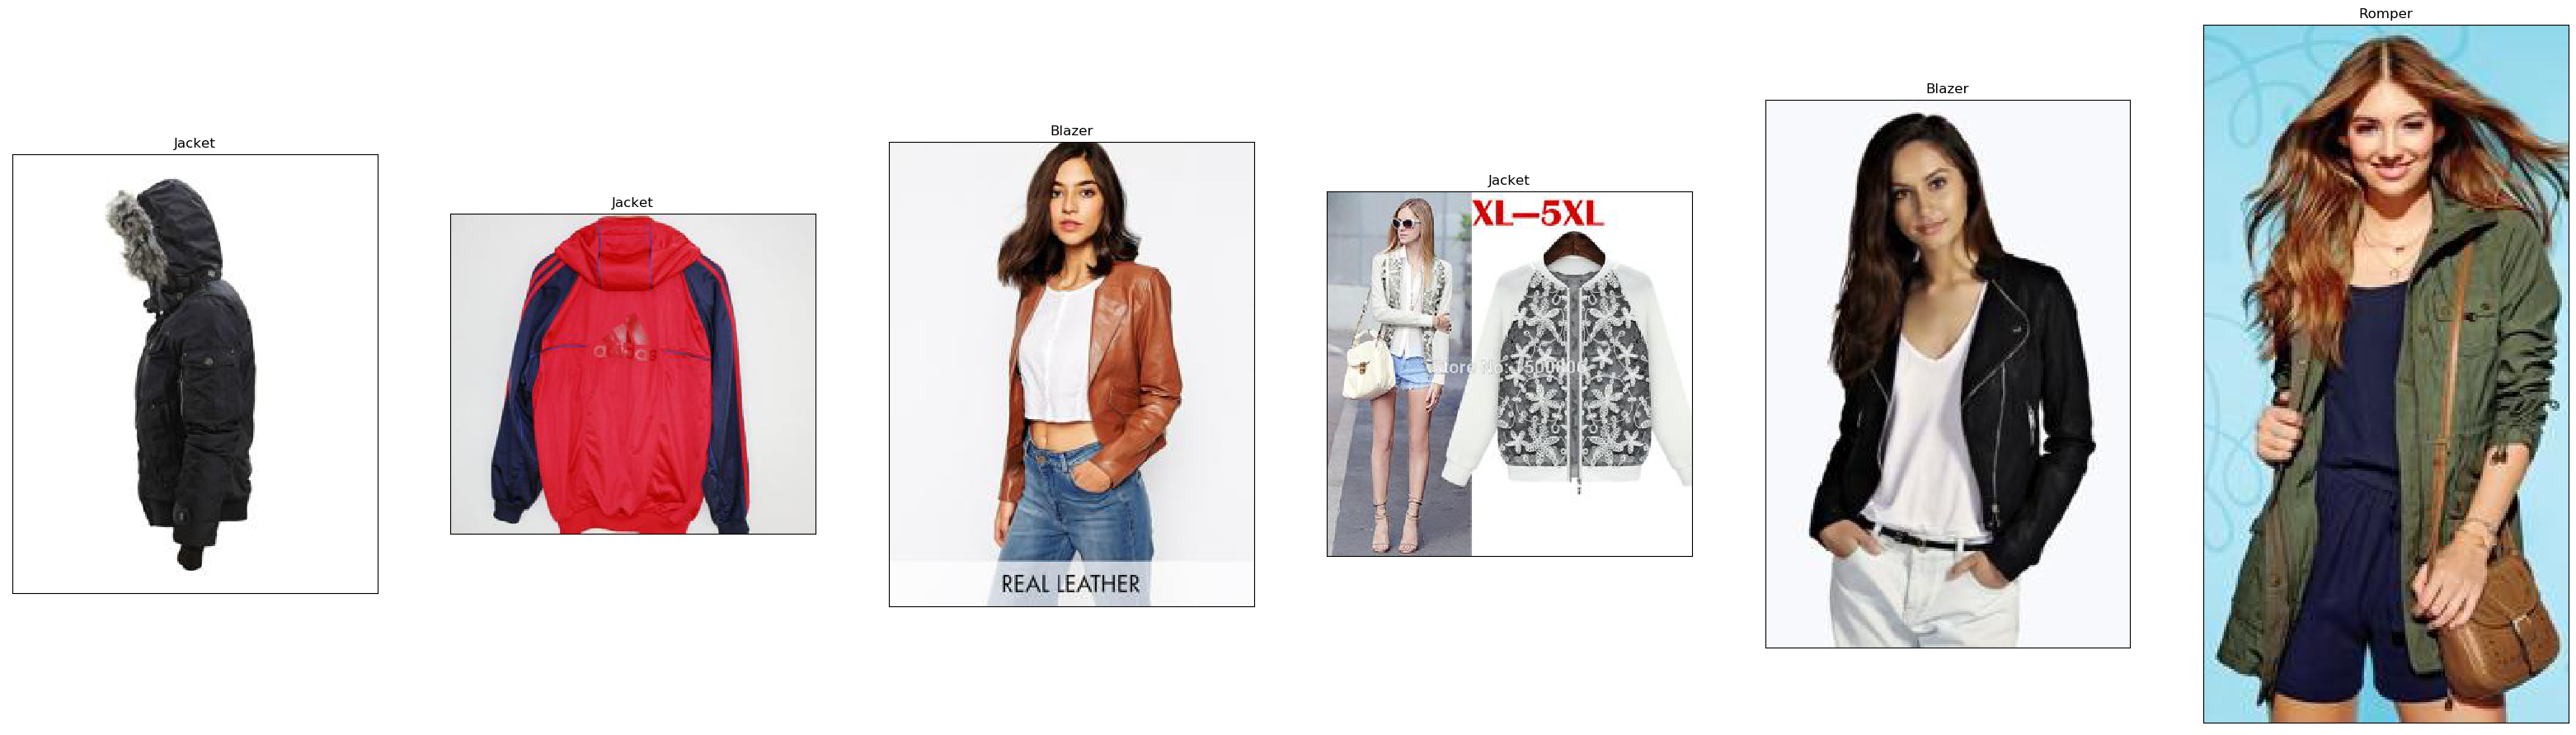
\includegraphics[width = 5in]{c/search_idx_3013.png}}\\
{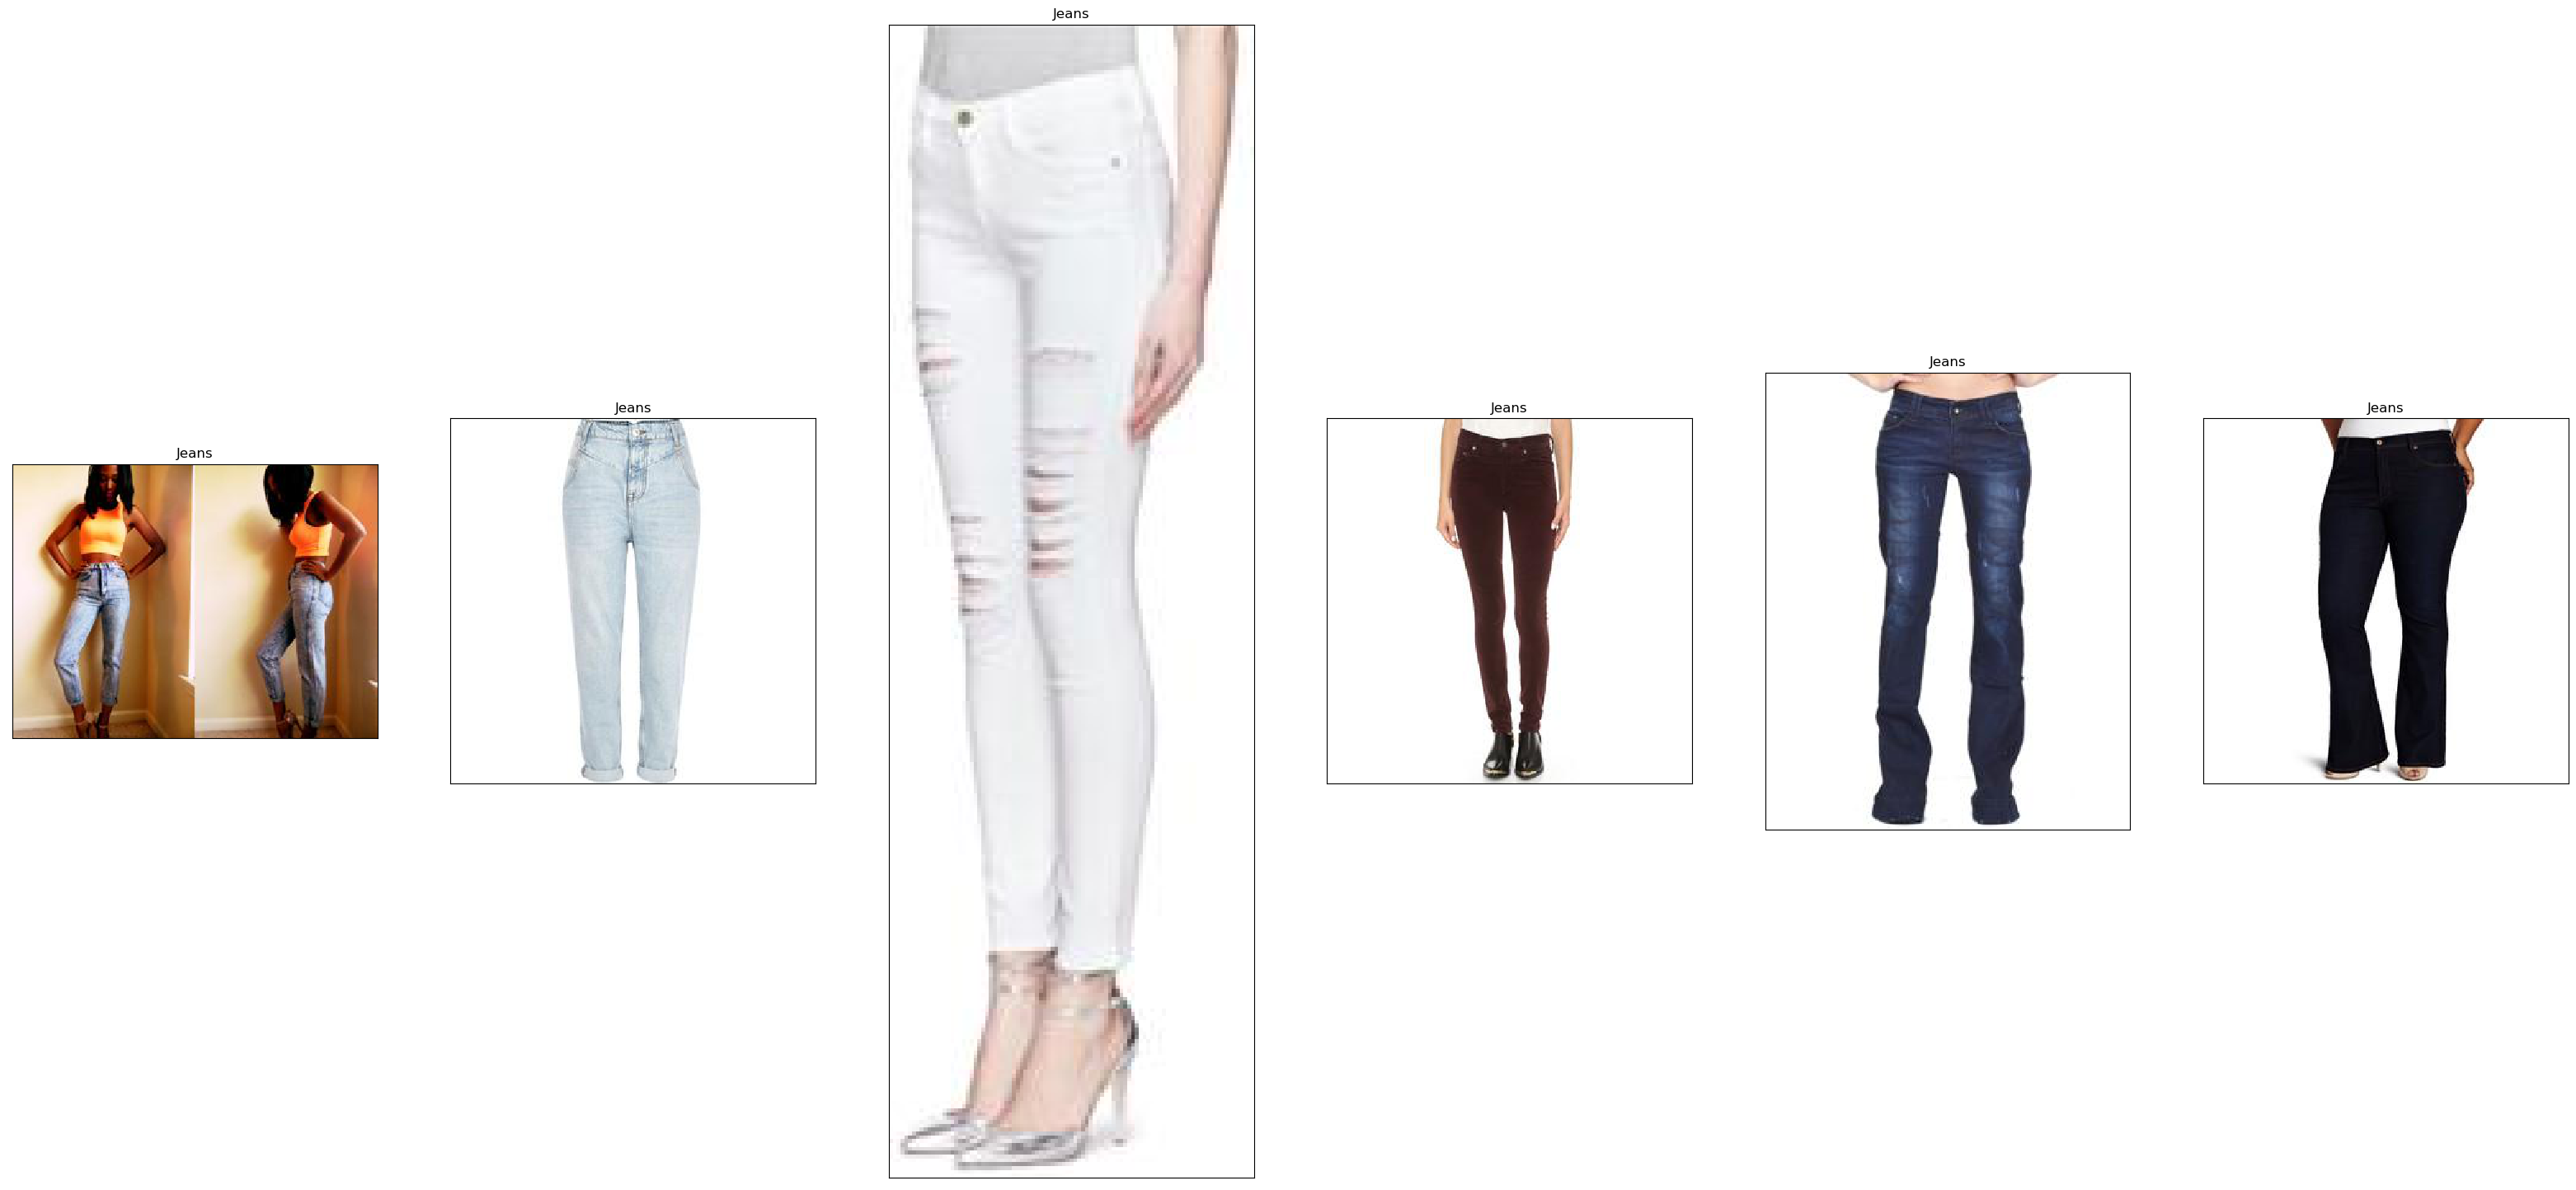
\includegraphics[width = 5in, height = 1.5in]{c/search_idx_4002.png}}\\
{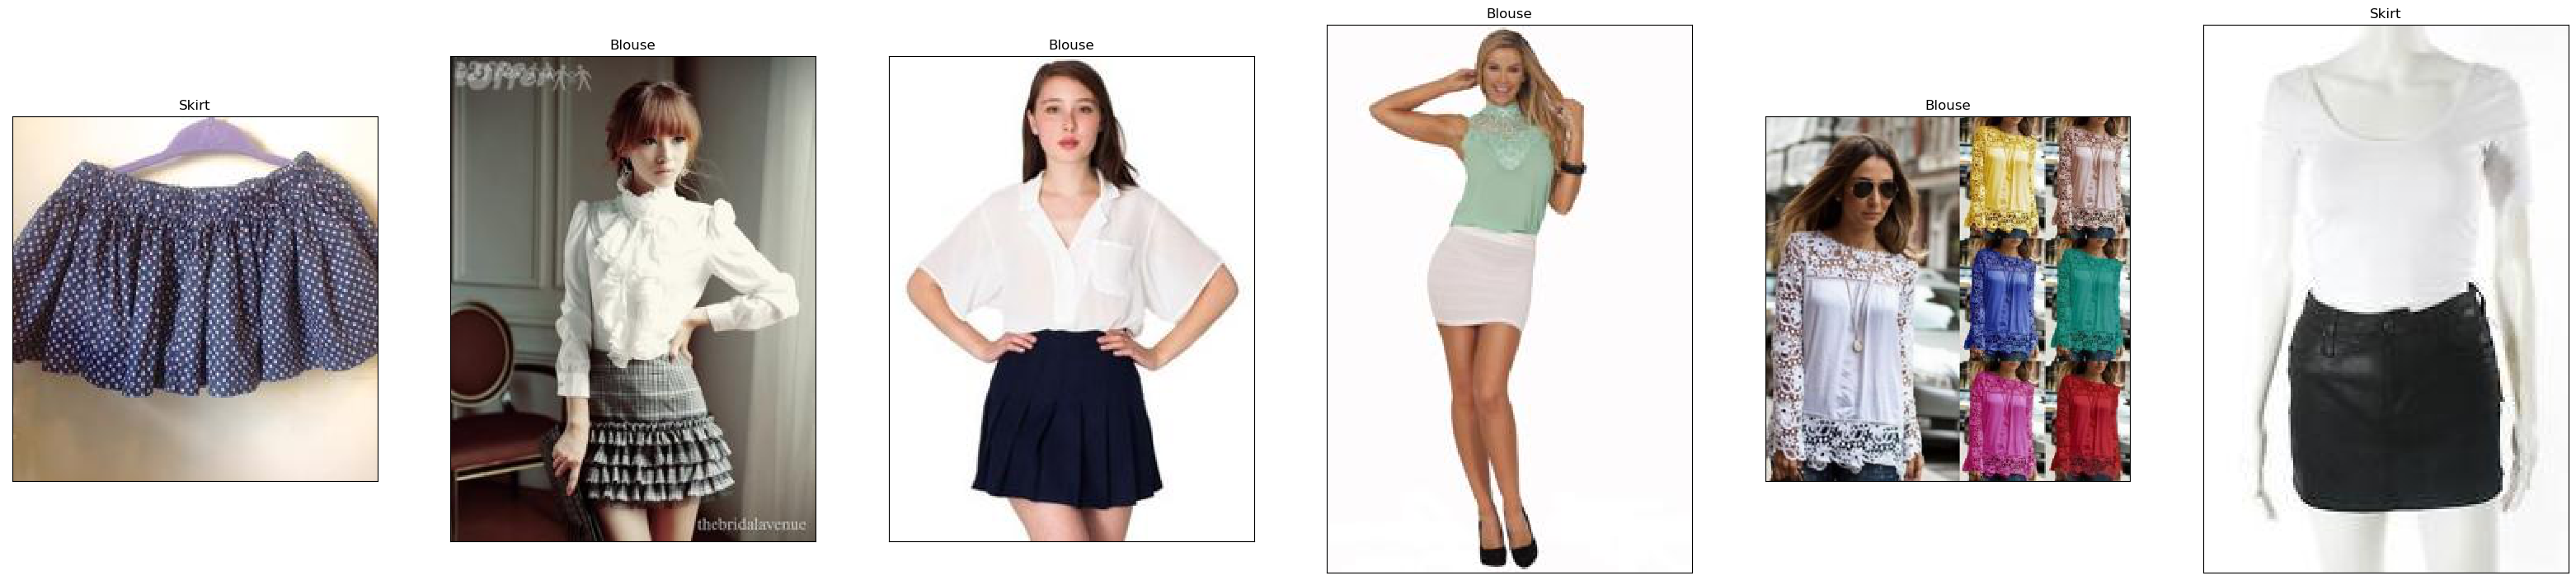
\includegraphics[width = 5in, height = 1in]{c/search_idx_7513.png}}\\
{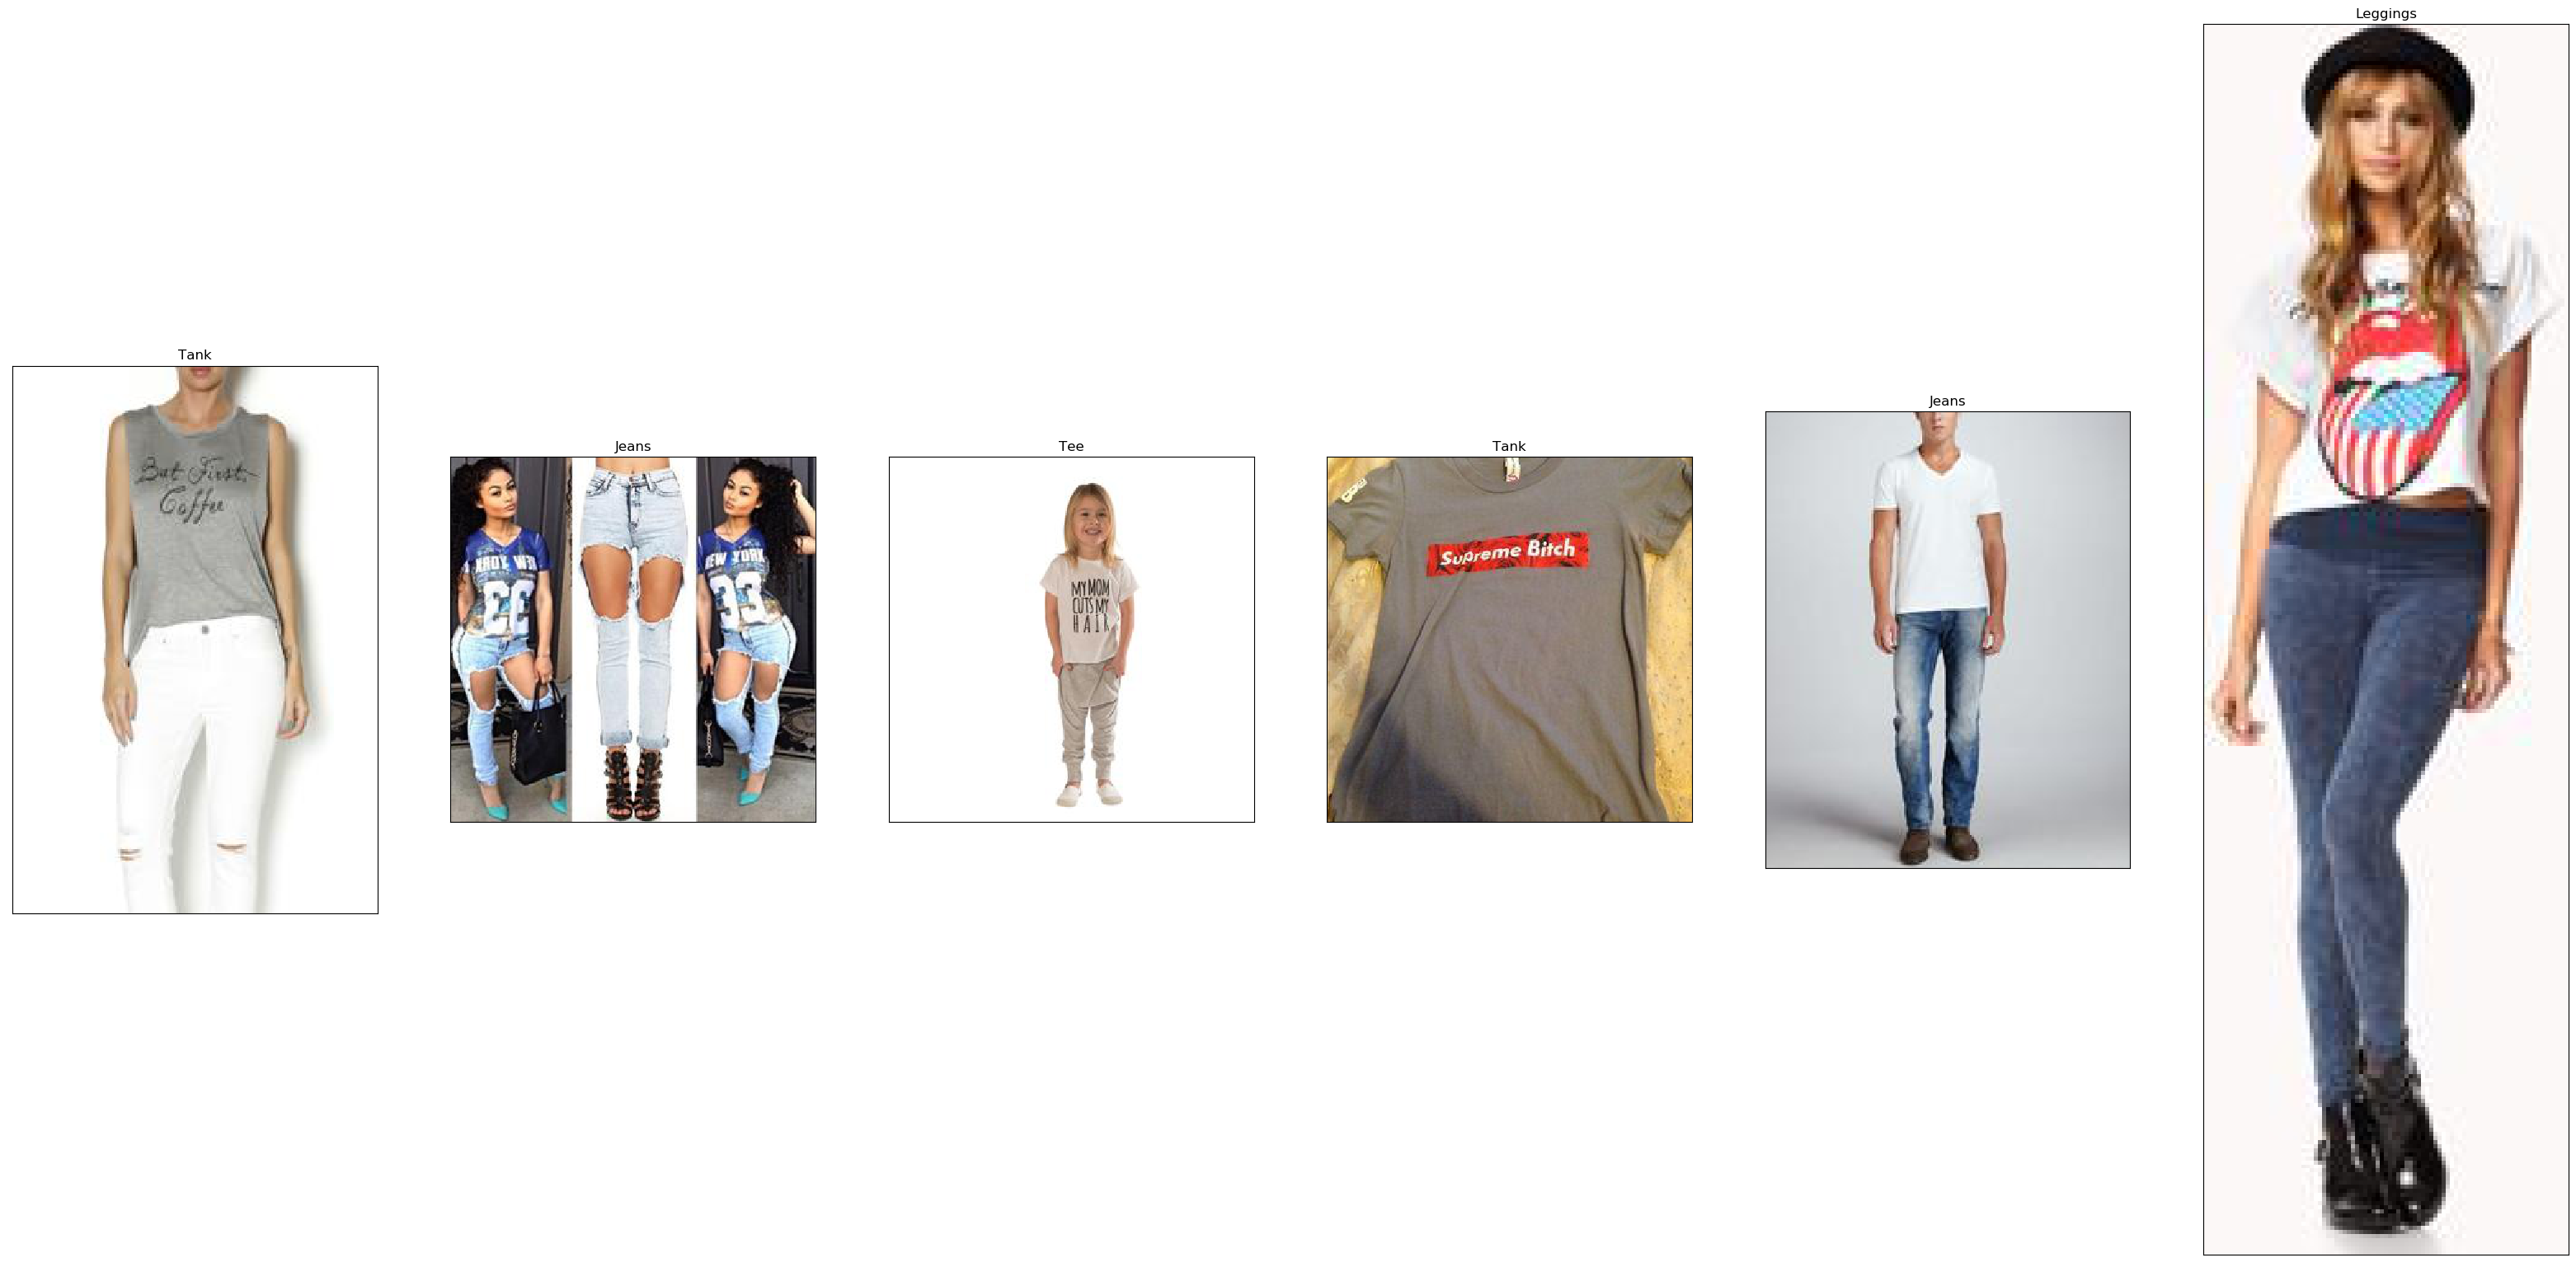
\includegraphics[width = 5in, height = 1.5in]{c/search_idx_8716.png}}\\
{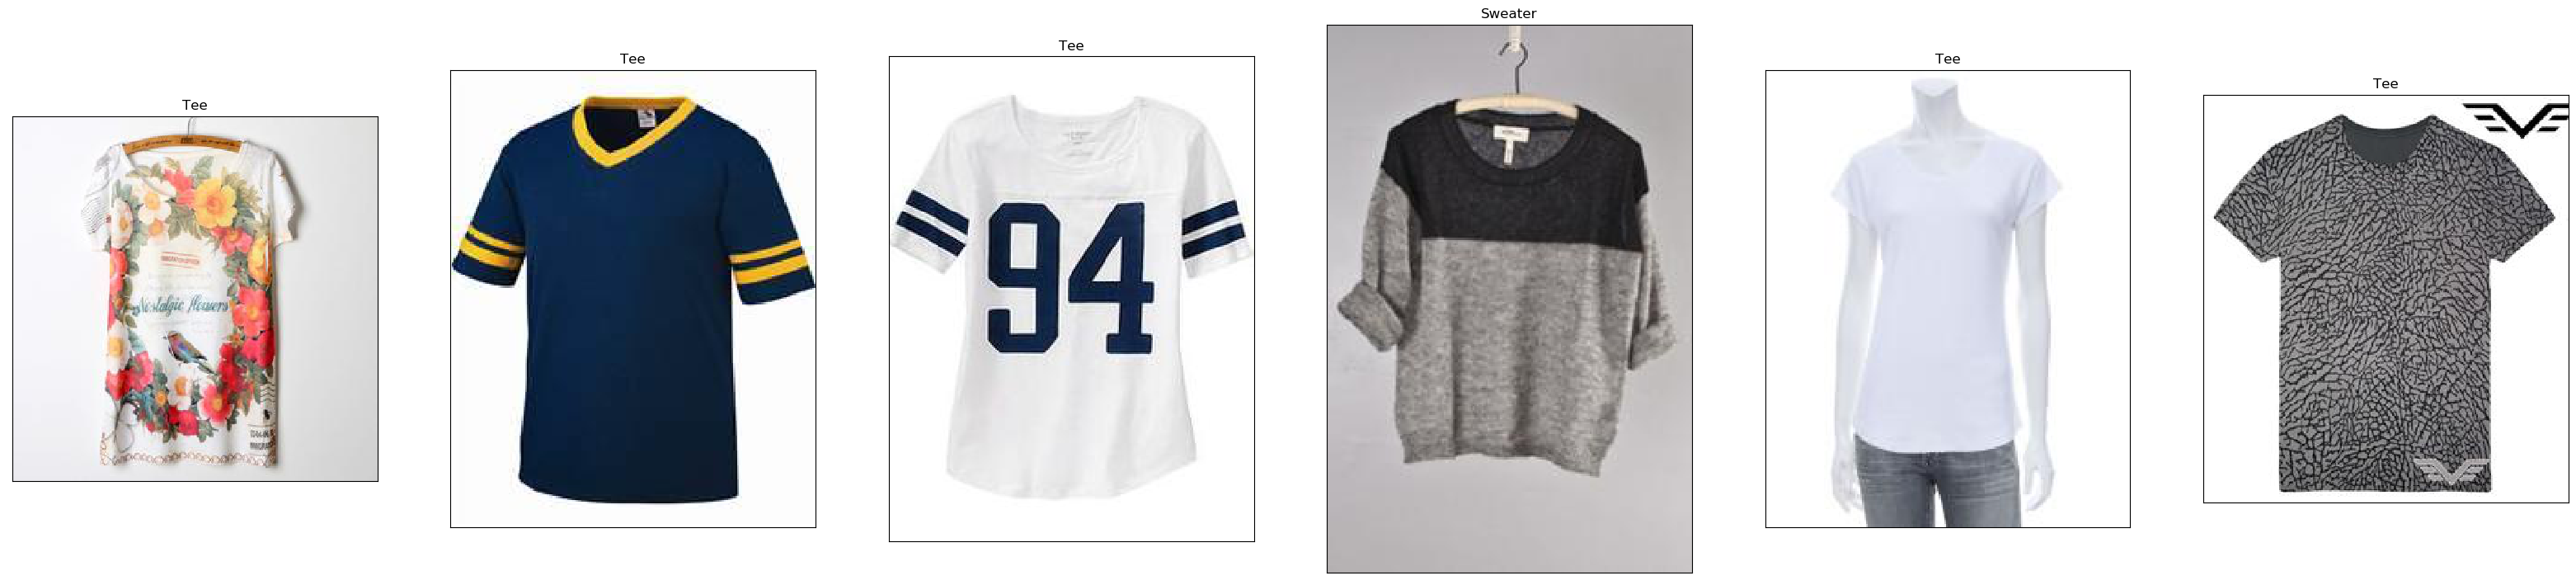
\includegraphics[width = 5in]{c/search_idx_9388.png}}
\end{tabular}
\caption{Top 5 images for Network (C)}
\label{fig:img_netC}
\end{figure}

\begin{figure}
\begin{tabular}{c}
{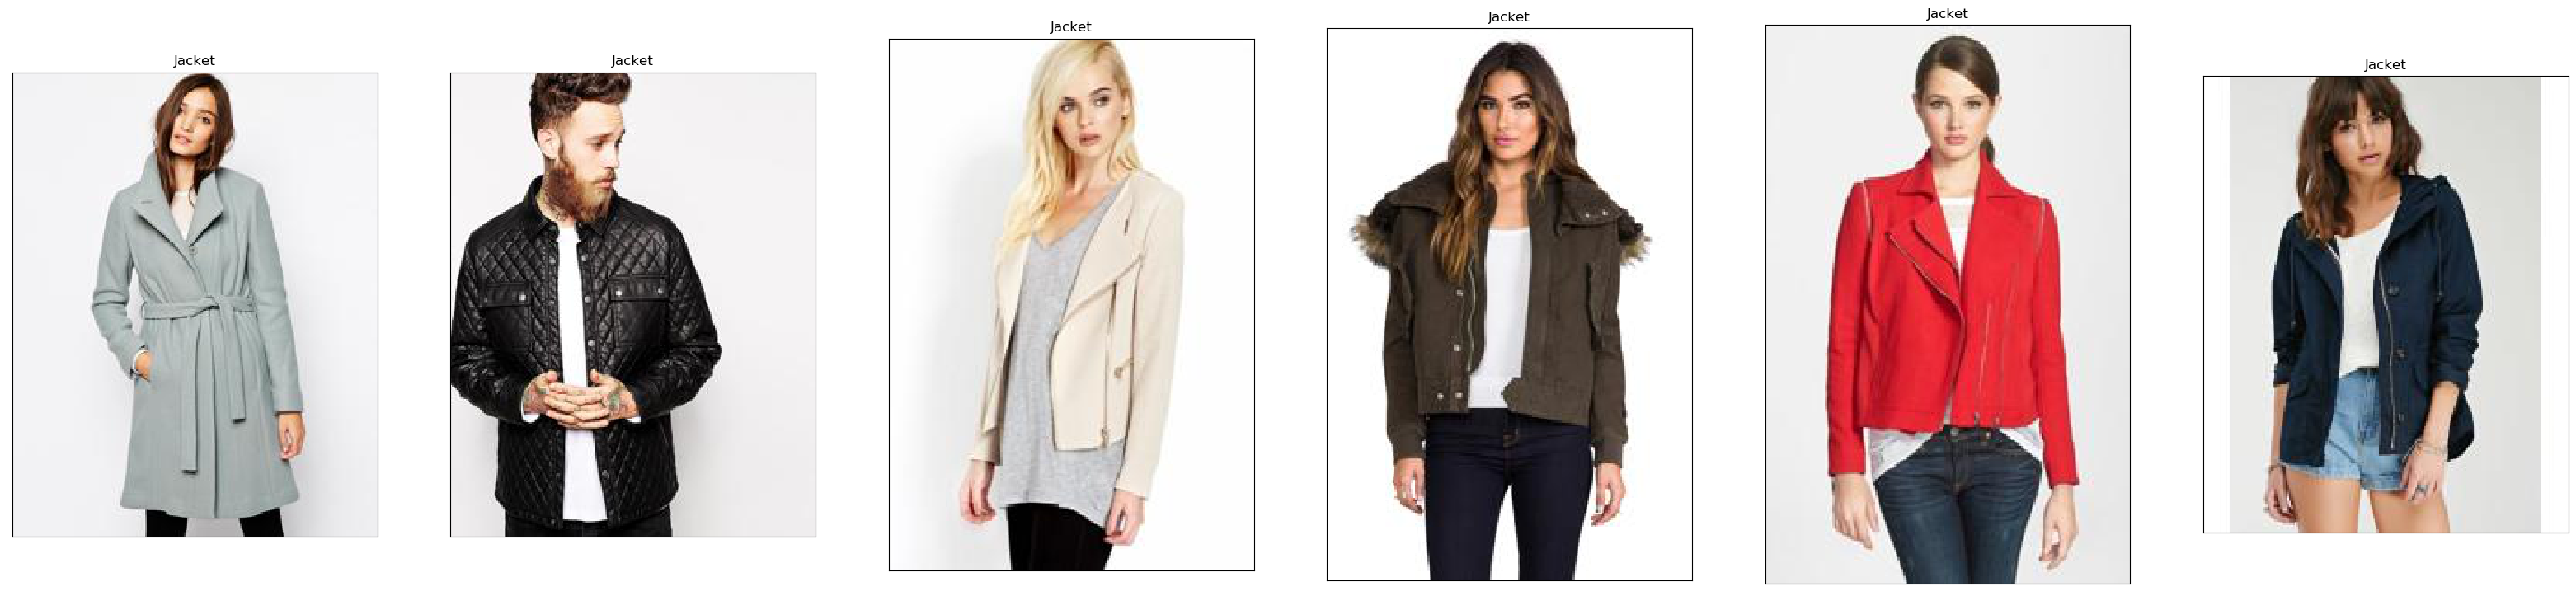
\includegraphics[width = 5in]{d/search_idx_3012.png}}\\
{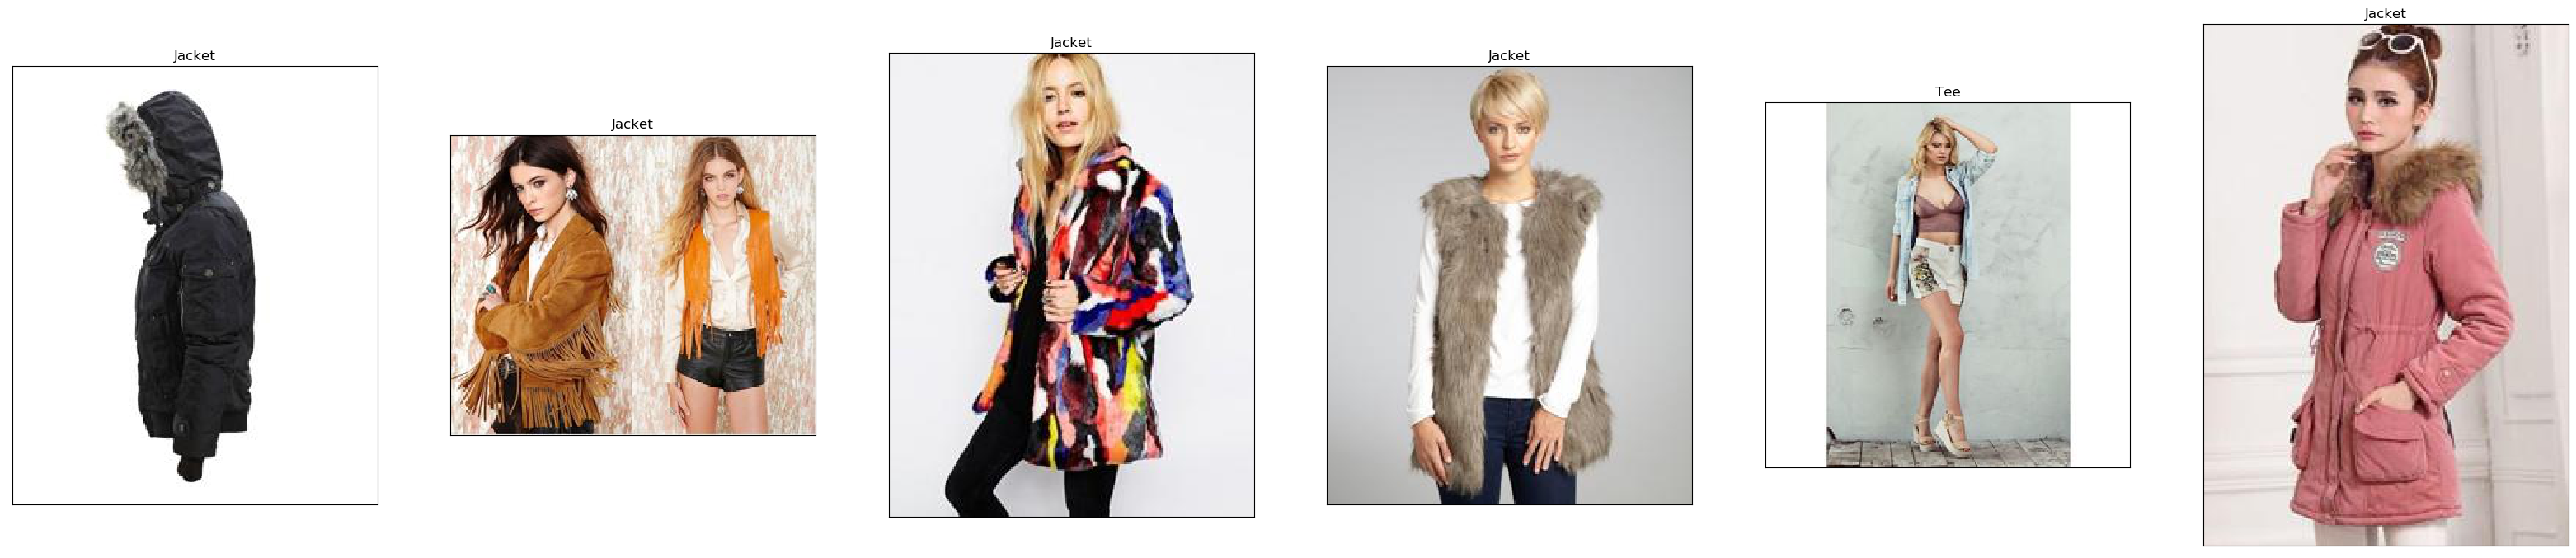
\includegraphics[width = 5in]{d/search_idx_3013.png}}\\
{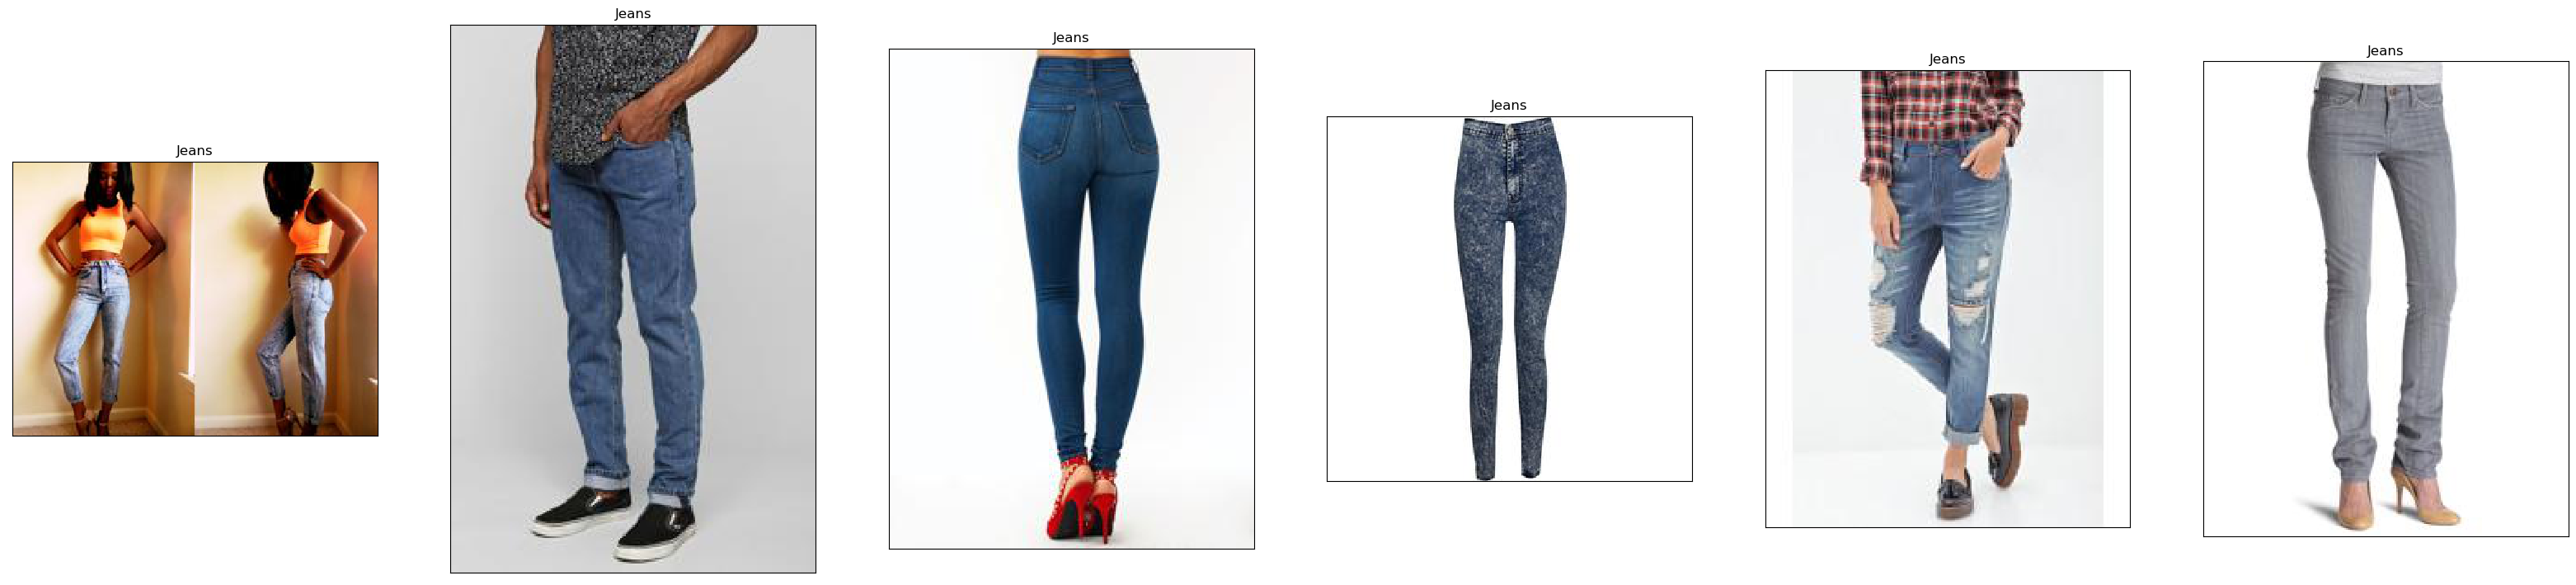
\includegraphics[width = 5in]{d/search_idx_4002.png}}\\
{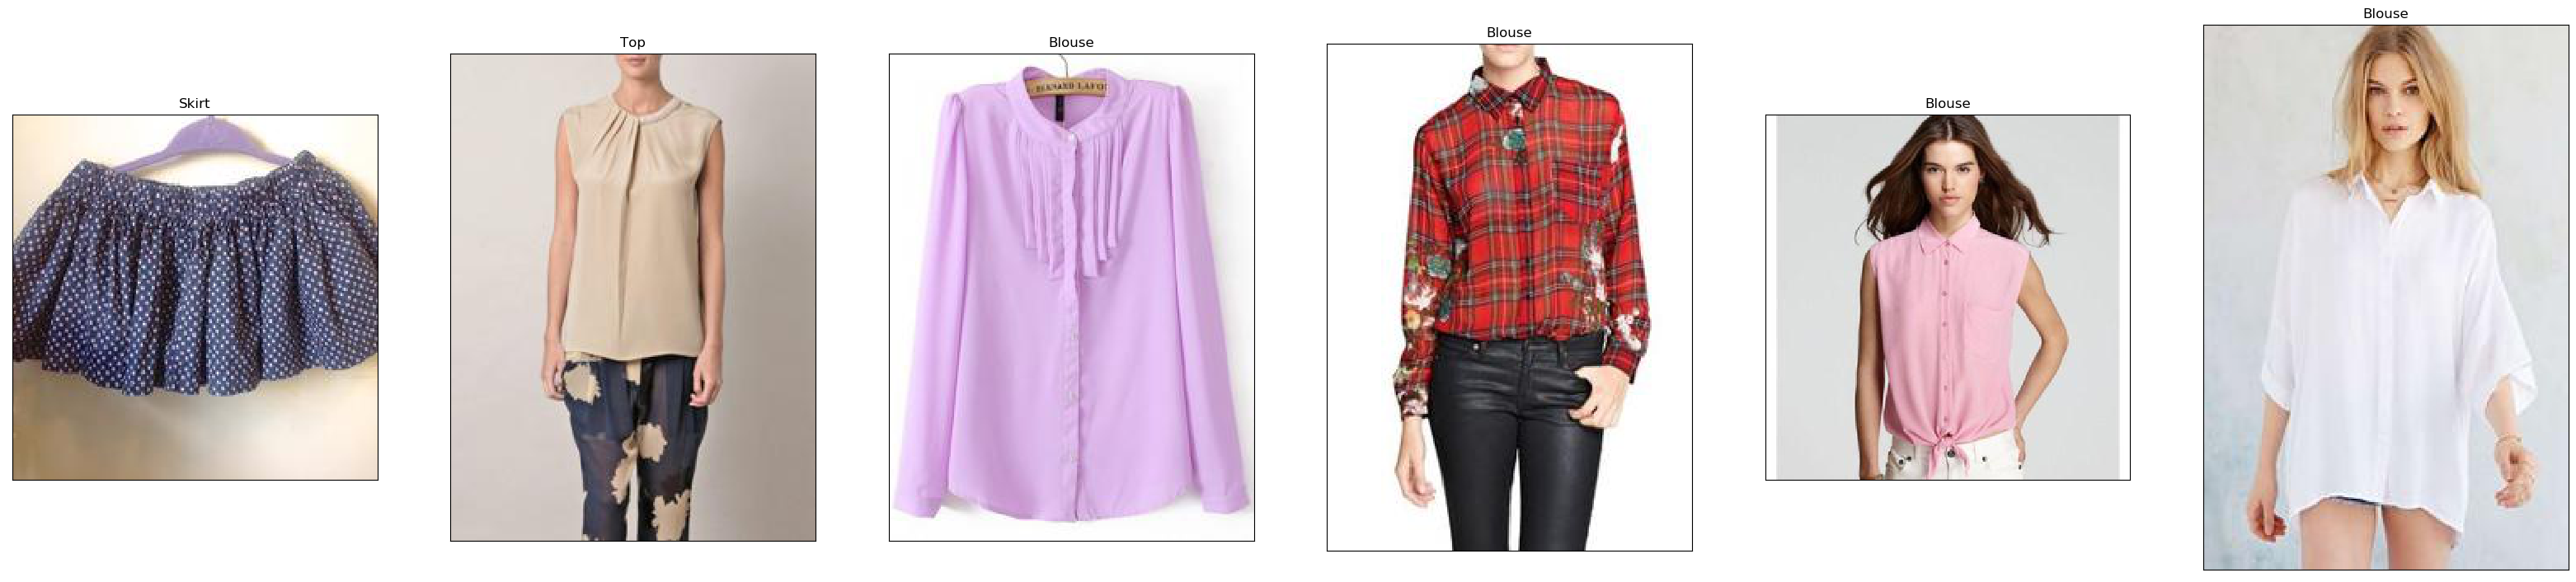
\includegraphics[width = 5in]{d/search_idx_7513.png}}\\
{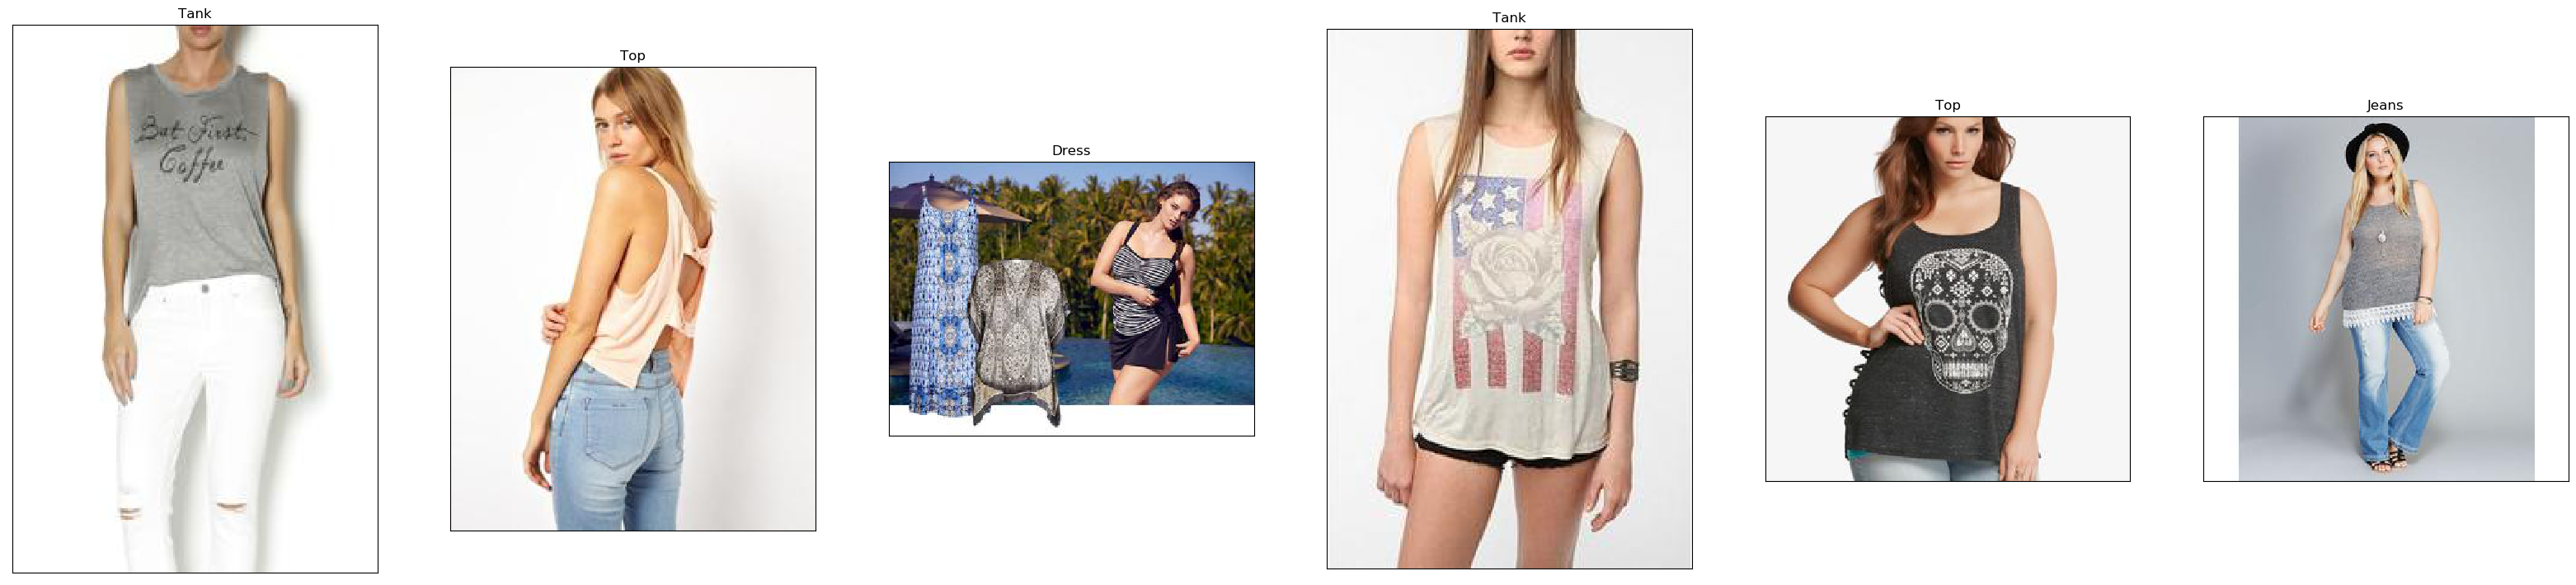
\includegraphics[width = 5in]{d/search_idx_8716.png}}\\
{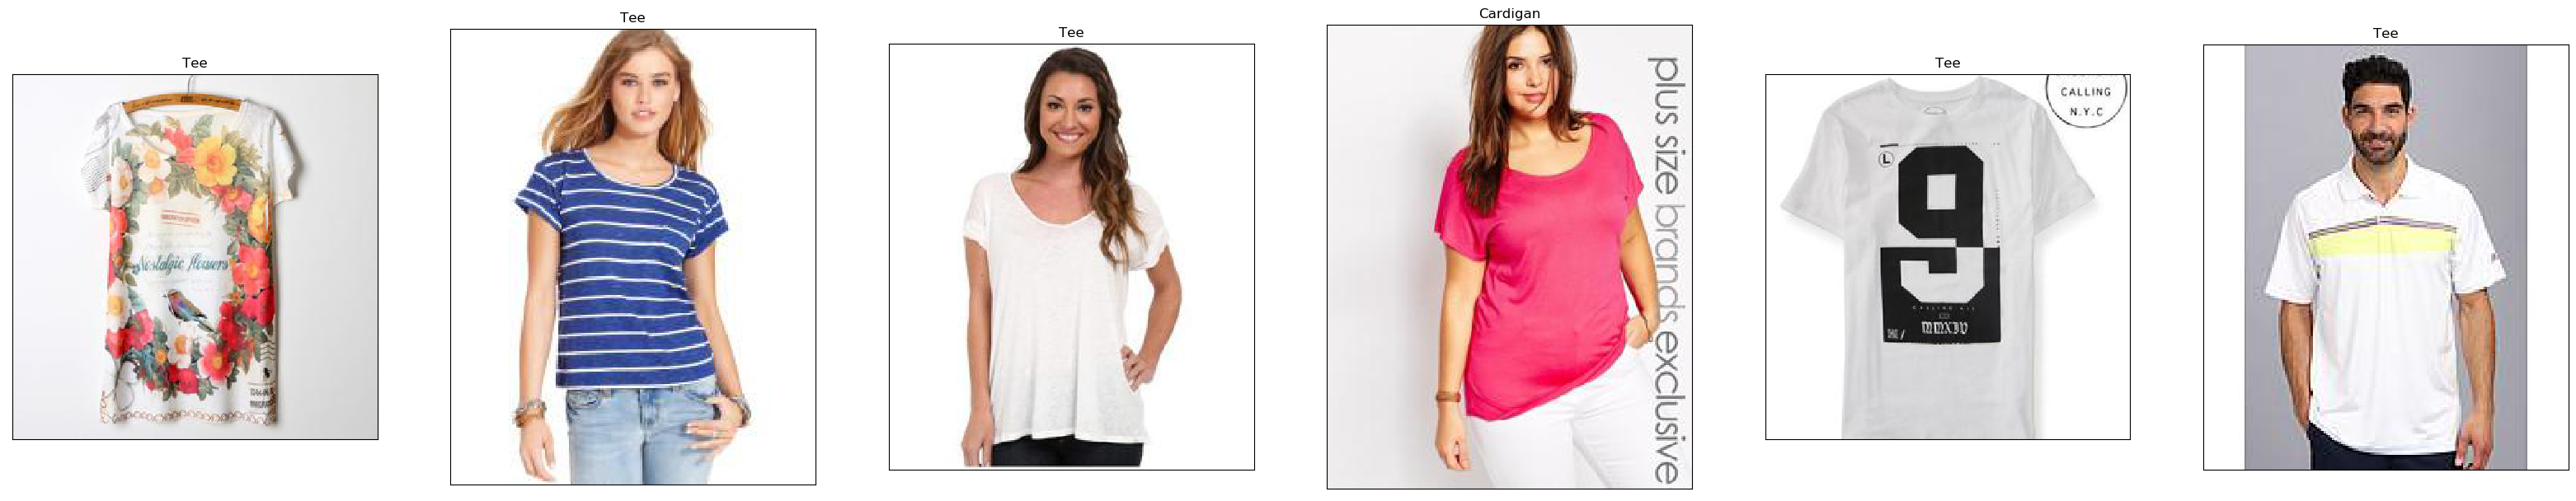
\includegraphics[width = 5in]{d/search_idx_9388.png}}
\end{tabular}
\caption{Top 5 images for Network (D)}
\label{fig:img_netD}
\end{figure}

\begin{figure}
\begin{tabular}{cc}
{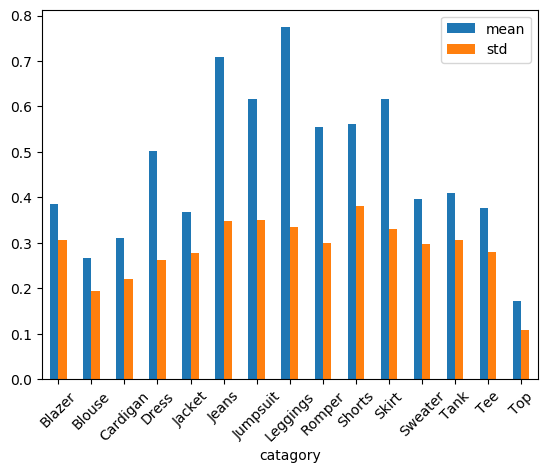
\includegraphics[width = 2.5in]{acc_plots/A_acc.png}} &
{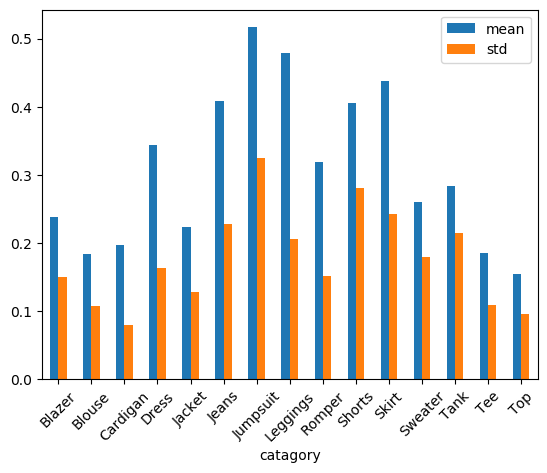
\includegraphics[width = 2.5in]{acc_plots/B_100_acc.png}} \\
A & B \\[6pt]
{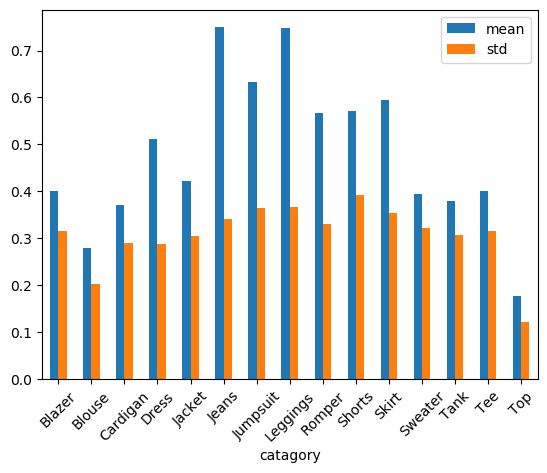
\includegraphics[width = 2.5in]{acc_plots/C_100_acc.png}} &
{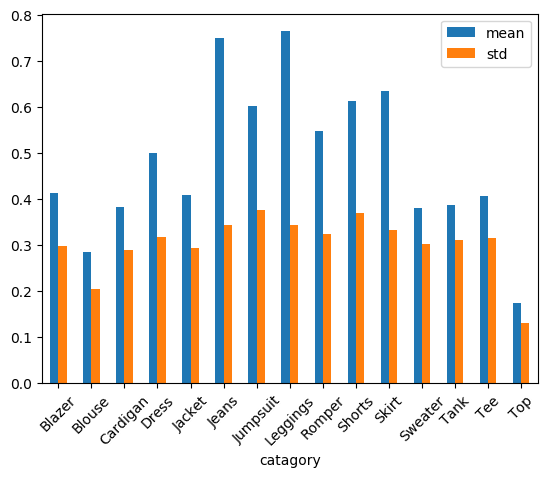
\includegraphics[width = 2.5in]{acc_plots/D_acc.png}} \\
C & D \\[6pt]
\end{tabular}
\caption{Top 50 accuracy per class for each network}
\label{fig:img_netD}
\end{figure}

\section{Discussion}
% Please reference to the artical two and write something

%   1. As the contractive loss term and the cs term are in the same other, the learning rate we used
%   in catagorial training can be also used in the siams+cos.

% See the exAMPLE below, we have +ve example and -ve example
% https://gits-15.sys.kth.se/chlin3/data-science-project-image-similarity/blob/master/exp_results/exp_siamese_m2_1000/search_idx_7513.png
% https://gits-15.sys.kth.se/chlin3/data-science-project-image-similarity/blob/master/exp_results/exp_siamese_m2_1000/search_idx_3013.pdf
The top 50 accuracy for each of the 4 networks are shown in Figure 17. Network B has the worst performance, networks A and C have similar performance, while network D has the best performance (slightly better than A and C). Therefore we conclude that Siamese network with class labels and embeddings regularisation has the best performance. Also, certain classes such as jeans, jumpsuit and leggings have better top 50 accuracies than the others. This is likely due to their more unique shapes or larger area compared to other classes such as tee, top and shorts. As we can see from Figure 17, this trend is consistent across all four networks.

Also in terms of visualization, we see that networks using both contrastive loss and class labels (C and D) form well separated clusters relatively. We also notice that in all embedding space visualizations, the class \textit{Top} is spread all across various other clusters. This was again very expected behaviour considering we define similarity by class label and \textit{Top} could be very well similar to other classes representing upper-wear. Another interesting comparison is between network B which uses only contrastive loss and networks C & D which use cross-entropy losses along with contrastive loss. We see less clusters in the network B as it clubs similar looking classes like Jeans and Leggings, since it doesn't account for class label explicitly. Network A which uses only cross-entropy loss also seperates classes well but it places them very close to each other as it doesn't account for distance between clothes.

Overall, network D is robust and can perform similarity queries better than networks A, B and C. There was no need to introduce additional hyperparameters to adjust the weighting between the entropy loss and the contrastive loss term, while for network C we needed to do this to achieve learning. One limitation of the data is that the image may contain all of a person's clothes and the environment while having the label of 'Jeans'. This causes noise to the network learning process. We believe that data preprocessing such as cropping the correct part of the image or shading out the environment would improve the accuracy of the models. Other deep learning methods such as Attention Mechanism could also improve the focus the learning on important parts of the image.




\section{Summary}

In this project, we focused on different model designs to explore the problem of image similarity. We tried Siamese networks with different losses as described in \cite{bell2015learning} for our experiments on DeepFashion-1 dataset. We tried various hyper-parameters to tune the network individually. We used dimensionality reduction methods and faster approximate nearest neighbour methods to evaluate the models. We also used qualitative human-eye evaluation of nearest retrieved images and visualized thee embedding space. 

Our result is that Siamese network with L2 normalized embeddings offer a relatively better clustering of similar images compared to other models. Despite that, we do recommend more rigourous testing through different similarity definitions other than just the class label for training. 

For example, similarity can be defined as sub-types within a class (blue pens or red pens), or even similar items across different classes (bicycle wheels and car wheels). In addition, different types of losses used for similarity comparison could be explored, such as triplet loss. Finally, other models such as autoencoders can be used to construct the embedding space instead of the Siamese model.

\subsection{Insights from Other Group}
We met group 9 who were also working on the Image Similarities project. During the course our discussion we explained our respective implementations to each other. Apart from the use of Siamese networks, our approaches to the problem are very different. They were using a different non-DeepFashion dataset and in total had 6 classes and 15000 images, but their use of triplets offers them as many training samples as they want. We use pairs instead of triplets and had significantly more classes and images in the dataset. Another significant difference was how we defined similarity, they had different versions of same cloth and it forms their similarity but in our case we define the class label as the similarity. We offered them our thoughts on their idea of making their images gray-scale and possible alternatives. Possibly the triplet loss can be explored in a future work for the DeepFashion dataset.


\subsection{How we distributed the project work to all group members}
In this project, all of us took part in all activities but with different amount of work in each activity. We mainly divided our work as follows:
\begin{itemize}
  \item Literature review - All four members
  \item Code - One main coder, one main reviewer, two other coders
  \item Report - Two main writers, two reviewers
  \item Presentation - One main creator, two reviewers
\end{itemize}



\medskip
% \small
% \pagebreak
\bibliographystyle{unsrt}
\bibliography{references}

\end{document}
